\documentclass[a4paper,11pt,DIV=15,openany]{scrbook}

\usepackage[version=3]{mhchem}
\usepackage[utf8]{inputenc}
\usepackage{mathpazo,listings,braket,fancyvrb,booktabs,mystuff,colortbl,lastpage,array,longtable,framed}
\usepackage[colorlinks=true,urlcolor=B,linkcolor=B,citecolor=R]{hyperref}
\usepackage{tikz,pgfplots}
\pgfplotsset{compat=1.3}

% fonts
\usepackage{pxfonts}
\renewcommand*{\sfdefault}{lmss}


% Bold caption labels
\setkomafont{captionlabel}{\bfseries}

% Paragraph settings
\setlength{\parindent}{0pt}
\setlength{\parskip}{\smallskipamount}
% use a different parsep for lists
\usepackage{enumitem}
\setlist[itemize]{parsep=0pt}
\setlist[enumerate]{parsep=0pt}

% no clubs and widows
\clubpenalty = 2000
\widowpenalty = 2000 
\displaywidowpenalty = 2000

% =============================== TITLE ==========================
\newenvironment{tpage}[3]{%
\KOMAoptions{twoside = false}
\addtokomafont{title}{\rmfamily}
  \begin{titlepage}
    \title{\hspace{1cm}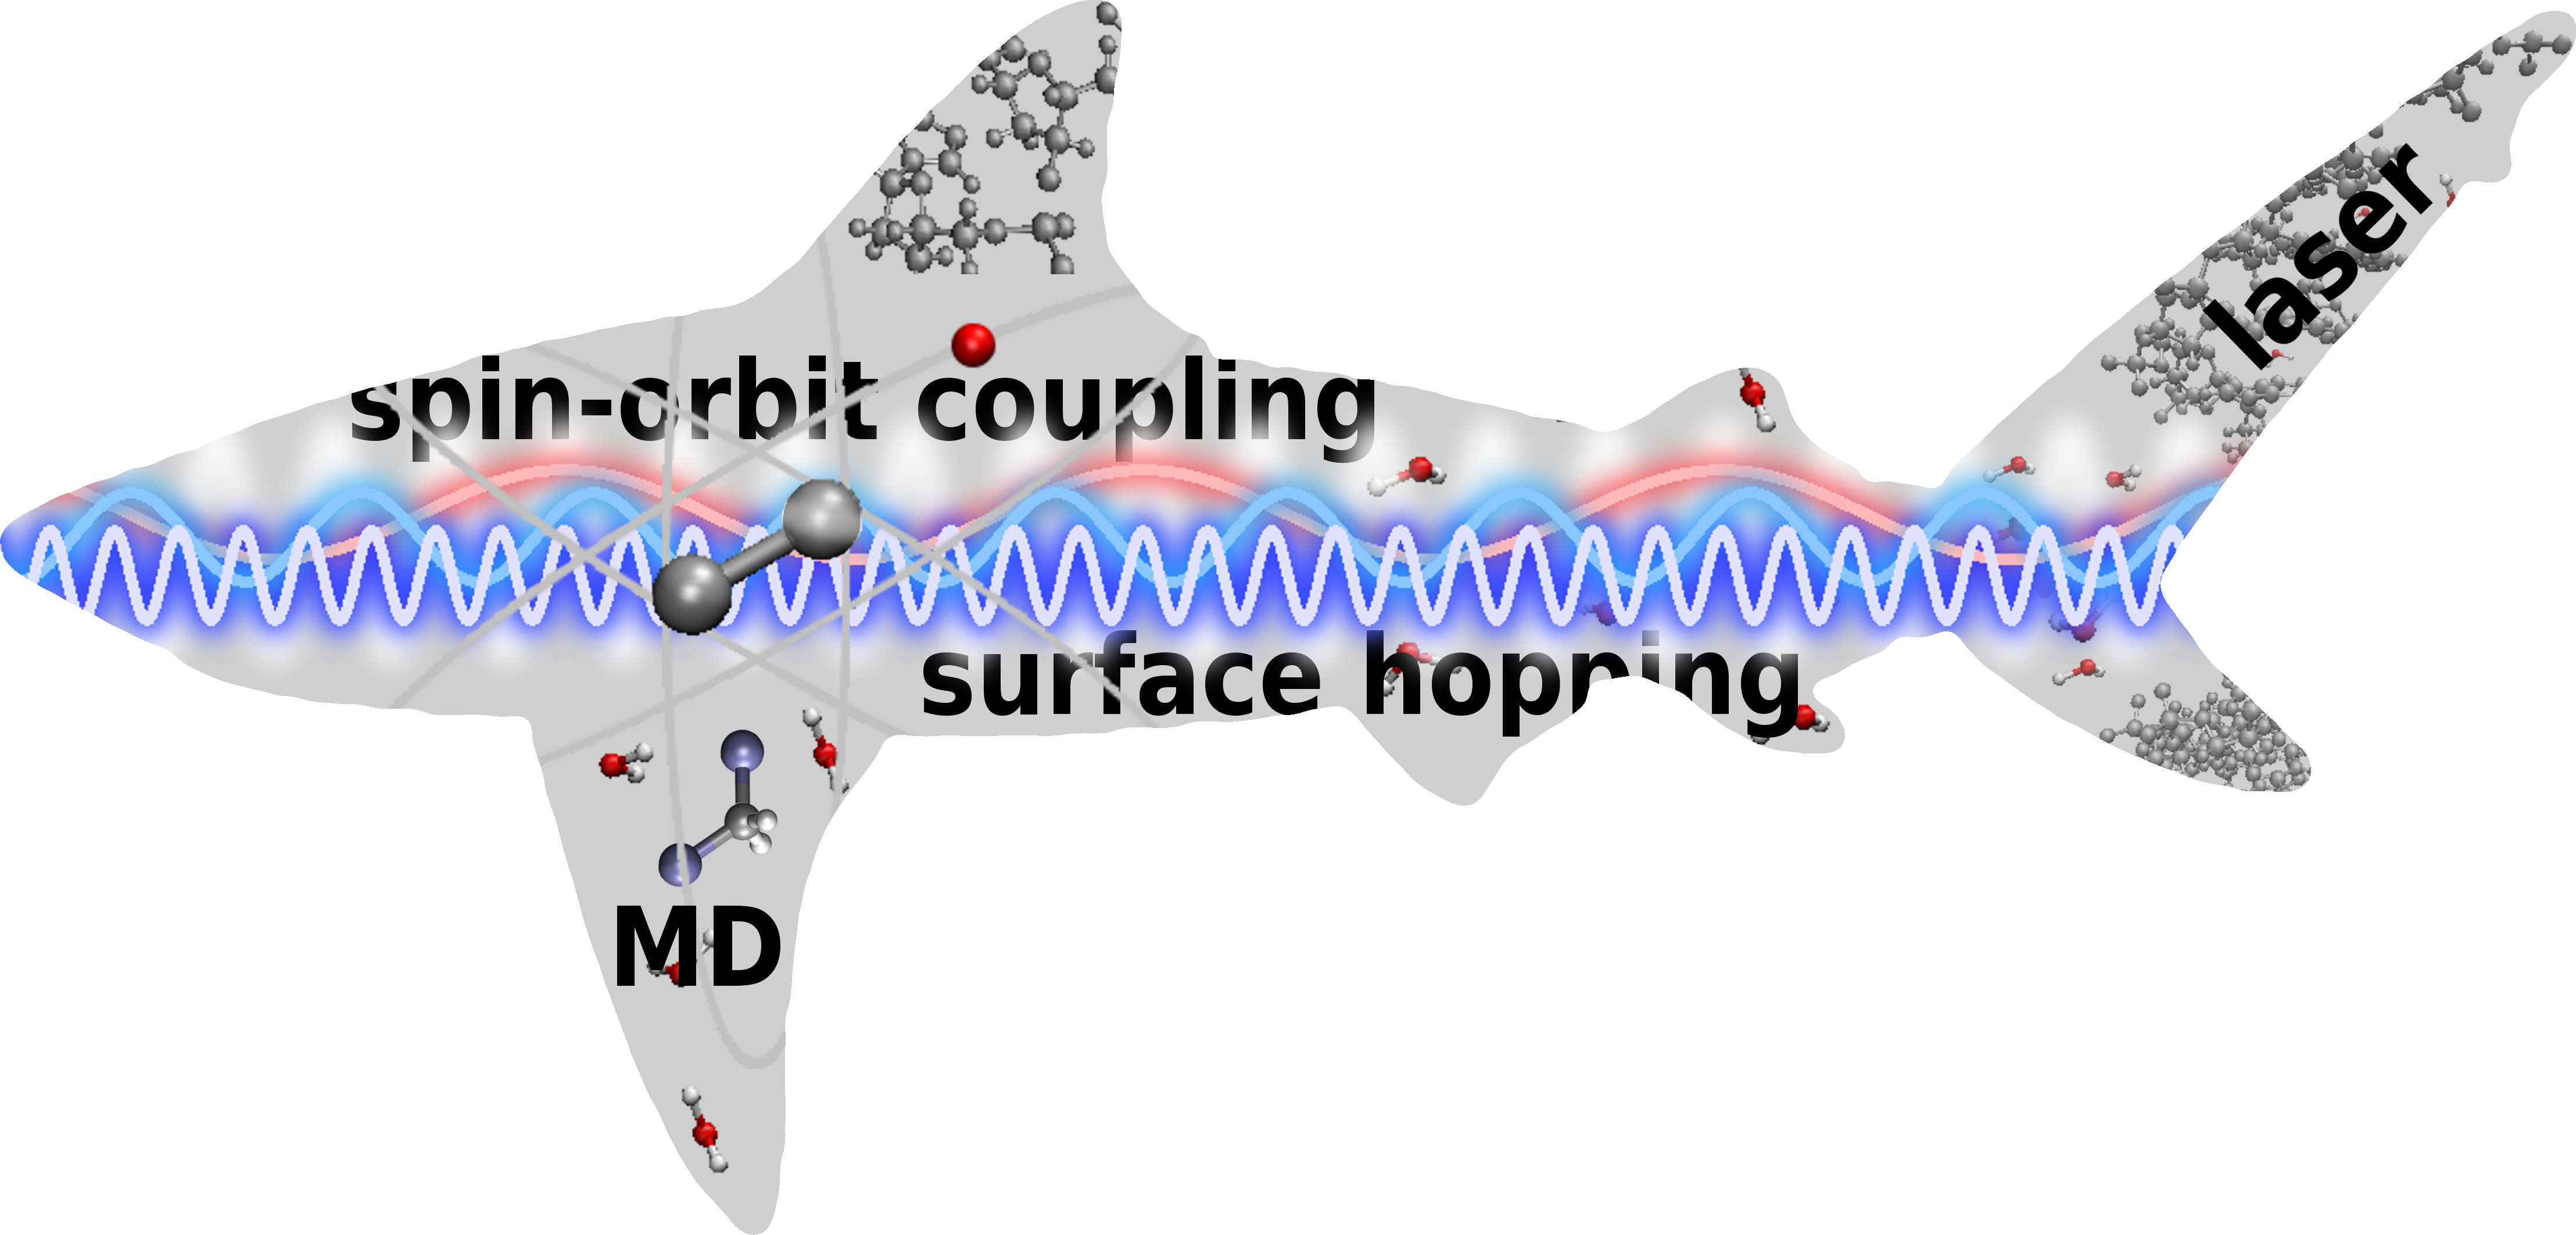
\includegraphics[width=0.8\textwidth,keepaspectratio=true]{img/sharc.png}\vspace{1.5cm}\\
    SHARC: Surface Hopping in the Adiabatic Representation Including Arbitrary Couplings}
    \subtitle{Tutorial}
    \date{Vienna, \today}
    \author{AG Gonz\'alez\\
Institute of Theoretical Chemistry\\
University of Vienna, Austria
\vspace{1cm}
% \\
% 
\includegraphics[width=0.25\textwidth,keepaspectratio=true]{img/logo.png}
\\

\includegraphics[width=0.4\textwidth,keepaspectratio=true]{img/univie.pdf}}

    \maketitle
  \end{titlepage}
\KOMAoptions{twoside = false}
}{}



% =============================== HEADER AND FOOT ==========================
\usepackage[automark]{scrpage2}
\pagestyle{scrheadings}
\clearscrheadfoot
\lehead{\leftmark}
\rehead{\rightmark}
\lohead{\leftmark}
\rohead{\rightmark}
\lofoot[Page \pagemark]{Page \pagemark}
\refoot[Page \pagemark]{Page \pagemark}




% =============================== KEYWORDS ==========================

\newcommand{\sharc}{\textsc{Sharc}}

\newcommand{\todo}[1]{\textcolor{RL}{#1}}

\newcommand{\dothis}[1]{#1}

\newcommand{\ttt}[1]{\texttt{#1}}

% shaded boxes
\definecolor{shadecolor}{HTML}{BBDDFF}

\newenvironment{example}{
  \vspace{0mm}
  \definecolor{shadecolor}{HTML}{E4F4FF}
  \begin{shaded}
}{
  \end{shaded}
}

% ========================================================================================================= %
% ========================================================================================================= %
% ========================================================================================================= %

\begin{document}

\tpage{Author}{Title}{Subtitle}

% ========================================================================================================= %
% ========================================================================================================= %
% ========================================================================================================= %

\tableofcontents
% \clearpage

% ========================================================================================================= %
% ========================================================================================================= %
% ========================================================================================================= %

\chapter{Before you Start}

In this tutorial, the steps necessary to perform non-adiabatic dynamics with \sharc\ are explained. 
The tutorial consists of three tutorial sections. 

\textbf{The first one} is a quick tutorial, showing just the minimum steps necessary to run the dynamics code. 

\textbf{The second part} contains the full tutorial presenting a complete dynamics study including initial condition generation and trajectory analysis (with plotting of the results and a brief discussion). 

\textbf{The third part} is a collection of more specialized tutorials showing some advanced usage aspects in detail.

At the end of this document, some additional hints for the usage of the quantum chemistry interfaces are given.




\section{Description of the model system}

The task of the tutorial is to simulate the excited-state dynamics of ethylene. The employed method will be CASSCF(2,2)/6-31G*, using the \textsc{Molpro} program package. It is known that the excited-state manifold of ethylene necessitates a much more complex electronic structure treatment than CASSCF(2,2). Nevertheless, for the purposes of this tutorial it is sufficient to use the mentioned CASSCF method.

The main idea is to simulate the well-known excited-state dynamics of ethylene, which after excitation to the $\pi\pi^*$ state undergoes torsion around the double bond. This leads to a conical intersection with the ground state, allowing for ultra-fast relaxation. Additionally, we will also include the triplet $\pi\pi^*$ state, which is possible with the \sharc\ methodology. However, since spin-orbit coupling is very weak in this system (only light atoms, El-Sayed-forbidden), we do not expect ISC to occur. 

In the following, an overview over the level of theory and the initial geometry are given:

\definecolor{shadecolor}{HTML}{BBDDFF}
\begin{example}
\begin{minipage}{0.45\textwidth}
  \centering
  Ab initio level of theory for ethylene.
  \begin{tabular}{ll}
    \toprule
    Molecule            &Ethylene\\
    Charge              &zero\\
    Program             &\textsc{Molpro}\\
    Method              &SA-CASSCF(2,2)\\
    Basis set           &6-31G*\\
    Number of states    &2 Singlets, 1 Triplet\\
    \bottomrule
  \end{tabular}
\end{minipage}
\hfill
\begin{minipage}{0.45\textwidth}
  \begin{verbatim}
6
Initial geometry ethylene
 C  0.000000  0.000000  0.000000
 C  0.000000  0.000000  1.335000
 H  0.943102  0.000000 -0.544500
 H  0.943102  0.000000  1.879500
 H -0.943102  0.000000  1.879500
 H -0.943102  0.000000 -0.544500
  \end{verbatim}
\end{minipage}
\end{example}


\chapter{Quick Tutorial}

Here we just present how to prepare a single trajectory, using the equilibrium geometry as starting geometry and random velocities. 

The goal is to prepare all input files for \sharc\ and the \textsc{Molpro} interface. The necessary files and directories are presented in figure~\ref{fig:traj_dir}. Note that the files \ttt{MOLPRO.template} and \ttt{SH2PRO.inp} are only necessary since we are using the \sharc-\textsc{Molpro} interface.

\begin{figure}
  \centering
  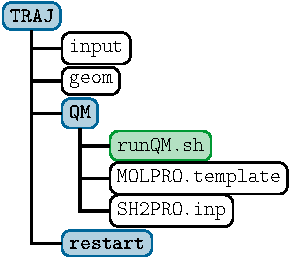
\includegraphics[]{img/dir_traj/dir_traj.pdf}
  \caption{Input files for a \sharc\ dynamics simulation.}
  \label{fig:traj_dir}
\end{figure}

The contents of the files are given in the following.

\section{Input File}

The \sharc\ input file (``\ttt{input}'') contains the dynamics settings and names of additional input files (geometry, velocity, coefficients). An example is given below:
\definecolor{shadecolor}{HTML}{BBDDFF}
\begin{example}\vspace{-8mm}
\begin{verbatim}
geomfile "geom"
veloc random 0.1

nstates 2 0 1 
state 2 mch
coeff auto

ezero -78.0814
tmax 10.0
stepsize 0.5

surf sharc
coupling ddr
\end{verbatim}\vspace{-5mm}
\end{example}

The meaning of these keywords is: The geometry is read from file \ttt{geom}. The nuclear velocities are picked at random, with 0.1 eV kinetic energy per atom. Two singlet states and one triplet state (with 3 components) will be included in the simulation. The initial state is the second state (the $S_1$). The initial coefficients will be set automatically (the initial state will get a coefficient of 1.0, the remaining state zero). The diagonal elements of the Hamiltonian will be shifted by -78.0814 Hartree. The simulation will include 10 fs, with a 0.5 fs timestep. The \sharc\ formalism will be used (propagation on the diagonalized states). Vectorial non-adiabatic couplings will be used for the propagation. 

\section{Geometry File}

The geometry file ``\ttt{geom}'' contains the chemical symbols, atomic charge, $x$, $y$ and $z$ coordinates and the relative atomic masses.

\definecolor{shadecolor}{HTML}{BBDDFF}
\begin{example}\vspace{-8mm}
\begin{verbatim}
C 6.0  0.0 0.0  0.0 12.000
C 6.0  0.0 0.0  2.5 12.000
H 1.0  1.7 0.0 -1.2  1.008
H 1.0  1.7 0.0  3.7  1.008
H 1.0 -1.7 0.0  3.7  1.008
H 1.0 -1.7 0.0 -1.2  1.008
\end{verbatim}\vspace{-5mm}
\end{example}

\section{QM Run Script}

At each timestep, \sharc\ writes the current geometry and different keywords to the file \ttt{QM/QM.in} and then calls \ttt{runQM.sh}. After this call is finished, \sharc\ reads the results of the quantum chemistry calculation from \ttt{QM.out}.

In most of the cases, in \ttt{runQM.sh} simply one of the \sharc-interfaces is called.
\definecolor{shadecolor}{HTML}{BBDDFF}
\begin{example}\vspace{-8mm}
\begin{verbatim}
cd QM
$SHARC/SHARC_MOLPRO.py QM.in > QM.log
\end{verbatim}\vspace{-5mm}
\end{example}
The interface will do all work necessary to produce the desired file \ttt{QM.out}.

\section{MOLPRO Template}

The \textsc{Molpro} interface needs as additional input file giving the settings for the electronic structure calculation. The file is called ``\ttt{MOLPRO.template}''.

\definecolor{shadecolor}{HTML}{BBDDFF}
\begin{example}\vspace{-8mm}
\begin{verbatim}
***
memory,12500,k
basis=6-31G*

{casscf
frozen,0
closed,7
occ,9
wf,16,1,0
state,2
weight,1,1
wf,16,1,2
state,1
weight,1
};
---
\end{verbatim}\vspace{-5mm}
\end{example}

\section{Interface Input}

The interface additionally needs some paths, which are read from ``\ttt{SH2PRO.inp}''.
\definecolor{shadecolor}{HTML}{BBDDFF}
\begin{example}\vspace{-8mm}
\begin{verbatim}
molpro $MOLPRO/molpro
scratchdir ./SCRA/
savedir ../restart/
\end{verbatim}\vspace{-5mm}
\end{example}

\section{Running \sharc}

The trajectory can then be started by simply executing:
\definecolor{shadecolor}{HTML}{BBDDFF}
\begin{example}\vspace{-8mm}
\begin{verbatim}
$SHARC/sharc.x input 
\end{verbatim}\vspace{-5mm}
\end{example}

\section{Output}

\sharc\ produces four output files, \ttt{output.log}, \ttt{output.lis}, \ttt{output.dat} and \ttt{output.xyz}. The file \ttt{output.log} contains mainly a listing of the chosen options and the resulting dynamics settings. At higher print levels, the log file contains also information per timestep. \ttt{output.lis} contains a table with one line per timestep, giving active states, energies and expectation values. \ttt{output.dat} contains a list of all important matrices and vectors at each timestep. This information can be extracted with \ttt{data\_extractor.x} to yield plottable table files. \ttt{output.xyz} contains the geometries of all timesteps (the comments to each geometry give the active state).





\chapter{Full Tutorial}\label{chap:full}

This tutorial presents all steps of a dynamics simulation. These steps include preparation steps like optimization and frequency calculation, generation of the Wigner distribution, calculation of the excited states of the Wigner distribution, initial state selection. It will be shown how to run the dynamics simulations. Also, trajectory analysis will be visited, including plotting of energies, populations, etc.\ of a single trajectory, calculation of internal coordinates, ensemble populations.


\section{Important}

Beyond the core dynamics program the \sharc\ suite contains a number of Python scripts allowing to perform various types of setup and analysis tasks. 
There are basically two types of these scripts.
Non-interactive scripts can be controlled by command-line arguments and options. Every non-interactive script can be called with the command line option \ttt{-h} in order to get a description of the functionality and possible options.
Interactive scripts ask the user for information about the task to be conducted (using features like auto-complete and default values), and only perform the task after the input has been completed. 

In the tutorial, the output of the interactive scripts is shown as in this example. 
\texttt{\textcolor{red}{\textbf{Red bold text}}} gives the input which the user has to type. 
\begin{oframed}
\footnotesize\begin{Verbatim}[commandchars=\\\{\}]
Type of calculation: \textcolor{red}{\textbf{2}}
Frequency calculation? [True] \textcolor{red}{\textbf{<ENTER>}}

Geometry filename: [geom.xyz] (autocomplete enabled) \textcolor{red}{\textbf{g<TAB>}}
Geometry filename: [geom.xyz] (autocomplete enabled) \textcolor{red}{\textbf{geom.xyz}}
\end{Verbatim}
\end{oframed}

\normalsize
During the interactive sessions, square brackets indicate that the question has a default answer, which can be used by just pressing ENTER. If filenames or directory paths need to be entered, auto-complete is active, which can be used by pressing TAB. Every interactive script upon completion also produces a file \ttt{KEYSTROKES.name}, which contains all user input for the last run.

\begin{shaded}
  Please make sure before starting that \ttt{\$SHARC} is set to the directory containing the \sharc\ scripts and executables.

  It is also advisable to set \ttt{\$MOLPRO} to the \textsc{Molpro} executable.
\end{shaded}




% \clearpage
\section{Optimization and Frequency calculation}

In general, the user is free to calculate the frequencies and normal modes with any quantum chemistry software and any method he sees fit. The user only has to provide a standard MOLDEN format file containing the results of the frequency calculation. However, usually it is advisable to calculate the frequencies at the same level of theory as the dynamics calculation. For the ethylene example, we will use the quantum chemistry method specified above. 

Create an empty directory. Prepare a geometry file called \ttt{geom.xyz} containing the given geometry.
\begin{Verbatim}[commandchars=\\\{\}]
user@host> \textcolor{red}{mkdir Ethylene}
user@host> \textcolor{red}{cd Ethylene}
user@host> \textcolor{red}{vi geom.xyz}
\end{Verbatim}

The \sharc\ suite comes with an input generator for \textsc{Molpro}, which produces input for single-point calculations, optimizations and frequency calculations. It can be invoked with
\begin{Verbatim}[commandchars=\\\{\}]
user@host> \textcolor{red}{$SHARC/molpro_input.py}
\end{Verbatim}
The script is interactive. Start the script and prepare an optimization plus frequency calculation on SA-CASSCF level. The script can also generate a Bash-script to instantly launch the \textsc{Molpro} calculation.

\begin{oframed}
\footnotesize\begin{Verbatim}[commandchars=\\\{\}]
  ================================================================================
||                                                                                ||
||                           MOLPRO Input file generator                          ||
||                                                                                ||
||                              Author: Sebastian Mai                             ||
||                                                                                ||
||                                   Version:0.2                                  ||
||                                    04.06.14                                    ||
||                                                                                ||
  ================================================================================

This script allows to quickly create MOLPRO input files for single-points calculations,
ground state optimizations, frequency calculations and SA-CASSCF calculations. 
It also generates MOLPRO.template files to be used with the SHARC-MOLPRO Interface.
  
---------------------Type of calculation--------------------

This script generates input for the following types of calculations:
  1       Single point calculations (HF, DFT, MP2, SS/SA-CASSCF)
  2       Optimizations & Frequency calculations (HF, DFT, MP2, SS/SA-CASSCF)
  3       MOLPRO.template file for dynamics (SA-CASSCF)
Please enter the number corresponding to the type of calculation.

Type of calculation: \textcolor{red}{\textbf{2}}                       \textcolor{blue}{# Anything after # is a comment}
Frequency calculation? [True] \textcolor{red}{\textbf{<ENTER>}}        \textcolor{blue}{# Opt + Freq}

--------------------------Geometry--------------------------

Please specify the geometry file (xyz format, Angstroms):
Geometry filename: [geom.xyz] (autocomplete enabled) \textcolor{red}{\textbf{<ENTER>}}    \textcolor{blue}{# use default "geom.xyz"}
Number of atoms: 6
Nuclear charge: 16

Enter the total (net) molecular charge:
Charge: [0] \textcolor{red}{\textbf{<ENTER>}}
Number of electrons: 16

Use standard masses (most common isotope)? [True] \textcolor{red}{\textbf{<ENTER>}}

-----------------------Level of theory----------------------

Supported by this script are:
  1       HF
  2       DFT (Only numerical frequencies)
  3       MP2 (Only numerical frequencies)
  4       SS-CASSCF
  5       SA-CASSCF (Only numerical frequencies)

Level of theory: \textcolor{red}{\textbf{5}}        \textcolor{blue}{# SA-CASSCF}

Please enter the basis set.
For SA-CASSCF Optimizations/Frequencies and SS-CASSCF Frequencies,
only segmented basis sets are allowed.
Common available basis sets:
  Pople:     6-31G**, 6-311G, 6-31+G, 6-31G(d,p), ...
  Dunning:   cc-pVXZ, aug-cc-pVXZ, cc-pVXZ-DK, ...    not available
  Turbomole: def2-SV(P), def2-SVP, def2-TZVP, ...
  ANO:       ROOS                                     not available
Basis set: \textcolor{red}{\textbf{6-31G*}}
Douglas-Kroll scalar-relativistic integrals? [True] \textcolor{red}{\textbf{<ENTER>}}

-----------------------CASSCF Settings----------------------

Number of active electrons: \textcolor{red}{\textbf{2}}
Number of active orbitals: \textcolor{red}{\textbf{2}}
Please enter the number of states as a list of integers
e.g. 3 0 3 for three singlets, zero doublets and three triplets.
Number of states: \textcolor{red}{\textbf{2 0 1}}
Accepted number of states: 2 0 1

Please specify the state to optimize
e.g. 3 2 for the second triplet state.
Root: [1 1] \textcolor{red}{\textbf{<ENTER>}}        \textcolor{blue}{# first singlet state}

---------------------------Memory---------------------------

Memory in MB: \textcolor{red}{\textbf{300}}

#########################Full input#########################        \textcolor{blue}{# this output is for debugging}

ltype            5
DK               True
basis            6-31g*
mem              300
cas.norb         2
maxmult          3
cas.nact         2
ctype            2
nelec            16
cas.nstates      [2, 0, 1]
geom             [['C', 0.0, 0.0, -0.002313], 
                  ['C', -0.0, 0.0, 1.337313], 
                  ['H', 0.931545, 0.0, -0.572106], 
                  ['H', 0.931545, 0.0, 1.907105], 
                  ['H', -0.931545, 0.0, 1.907105], 
                  ['H', -0.931545, 0.0, -0.572106]]
cas.root         [1, 1]
natom            6
ncharge          16
freq             True
nondefmass       False

Writing input to MOLPRO.input

Run script? [True] \textcolor{red}{\textbf{<ENTER>}}

-----------------------Path to MOLPRO-----------------------

Environment variable $MOLPRO detected:
$MOLPRO=/usr/license/molpro/molpros_2012_1_5_Linux_x86_64_i8/bin//molpro

Do you want to use this MOLPRO installation? [True] \textcolor{red}{\textbf{<ENTER>}}

----------------------Scratch directory---------------------

Please specify an appropriate scratch directory. This will be used to temporally store the integrals. 
The scratch directory will be deleted after the calculation. Remember that this script cannot check 
whether the path is valid, since you may run the calculations on a different machine. The path will 
not be expanded by this script.
Path to scratch directory: (autocomplete enabled) \textcolor{red}{\textbf{$TMPDIR/Ethylene/Opt}}

Writing run script run_MOLPRO.sh

Finished
\end{Verbatim}
\end{oframed}

\normalsize

Execute the run script.
\begin{Verbatim}[commandchars=\\\{\}]
user@host> \textcolor{red}{sh run_MOLPRO.sh}
\end{Verbatim}
This will produce the files \ttt{MOLPRO.out}, \ttt{freq.molden} and \ttt{wf}. The first file contains (among other things) the ground state minimum energy (should be $-78.08139491$ Hartree) and the vibrational wavenumbers. Check for any imaginary frequencies. There should be an output block like this in the output file:
\begin{oframed}
\footnotesize\begin{Verbatim}[commandchars=\\\{\}]
   Low Vibration      Wavenumber
        Nr             [1/cm] 
        1                0.00
        2                0.00
        3                0.00
        4                0.00
        5                0.00
        6                0.00

     Vibration        Wavenumber
        Nr             [1/cm] 
        1              885.91
        2              970.08
        3             1068.60
        4             1299.39
        5             1342.30
        6             1439.73
        7             1605.70
        8             1774.83
        9             3319.44
       10             3339.21
       11             3396.75
       12             3422.73
\end{Verbatim}
\end{oframed}

\normalsize
The \ttt{wf} file contains the CASSCF orbitals and can be used as starting orbitals for subsequent CASSCF calculations. The \ttt{freq.molden} is needed in the next step.

\clearpage
\section{Sampling from Wigner distribution}

In the next step, the initial coordinates and velocities need to be calculated from the harmonic frequencies and normal modes. The corresponding \sharc\ script can be executed by typing
\begin{Verbatim}[commandchars=\\\{\}]
user@host> \textcolor{red}{$SHARC/wigner.py -n 20 freq.molden}
\end{Verbatim}
The \ttt{-n} option is necessary to specify the number of initial conditions to be generated. Here, we generate 20 initial conditions. The output should look like this:
\begin{oframed}
\footnotesize\begin{Verbatim}[commandchars=\\\{\}]
Initial condition generation started...
MOLDEN file                  = "freq.molden"
OUTPUT file                  = "initconds"
Number of geometries         = 20
Random number generator seed = 16661

Geometry:
 C   6.0  -0.00000000   0.00000000  -0.00760978  12.00000000
 C   6.0   0.00000000   0.00000000   2.53039416  12.00000000
 H   1.0   1.73012211   0.00000000  -1.07271869   1.00782503
 H   1.0   1.73012212   0.00000000   3.59550308   1.00782503
 H   1.0  -1.73012211   0.00000000   3.59550308   1.00782503
 H   1.0  -1.73012212   0.00000000  -1.07271870   1.00782503
Assumed Isotopes: H-1 C-12 
Isotopes with * are pure isotopes.

Frequencies (cm^-1):
   1     885.9700
   2     970.0600
   3    1068.5700
   4    1299.2900
   5    1342.3400
   6    1439.6100
   7    1605.6600
   8    1774.6800
   9    3319.3700
  10    3339.1300
  11    3396.7200
  12    3422.7000
\end{Verbatim}
\end{oframed}

The results of the sampling are written to the file \ttt{initconds}. This file contains all necessary information for subsequent steps.

\normalsize





\clearpage
\section{Setting up the initial energy calculations}

In the next step, for each geometry an excited-state calculation has to be conducted in order to obtain the excitation energies and oscillator strengths. This calculations can be setup using the script \ttt{setup\_init.py}. 

\subsection{\textsc{Molpro} input template}

However, first we need to prepare the input for the \textsc{Molpro} excited-state calculation. Again launch the \textsc{Molpro} input generator:
\begin{Verbatim}[commandchars=\\\{\}]
user@host> \textcolor{red}{$SHARC/molpro_input.py}
\end{Verbatim}
Prepare a template file for the \sharc-\textsc{Molpro} interface.
\begin{oframed}
\footnotesize\begin{Verbatim}[commandchars=\\\{\}]
  ================================================================================
||                                                                                ||
||                           MOLPRO Input file generator                          ||
||                                                                                ||
||                              Author: Sebastian Mai                             ||
||                                                                                ||
||                                   Version:0.2                                  ||
||                                    04.06.14                                    ||
||                                                                                ||
  ================================================================================

This script allows to quickly create MOLPRO input files for single-points calculations,
ground state optimizations, frequency calculations and SA-CASSCF calculations. 
It also generates MOLPRO.template files to be used with the SHARC-MOLPRO Interface.
  
---------------------Type of calculation--------------------

This script generates input for the following types of calculations:
  1       Single point calculations (HF, DFT, MP2, SS/SA-CASSCF)
  2       Optimizations & Frequency calculations (HF, DFT, MP2, SS/SA-CASSCF)
  3       MOLPRO.template file for dynamics (SA-CASSCF)
Please enter the number corresponding to the type of calculation.

Type of calculation: \textcolor{red}{\textbf{3}}        \textcolor{blue}{# MOLPRO.template generation}

--------------------------Geometry--------------------------

No geometry necessary for MOLPRO.template generation

Number of electrons:  [16] \textcolor{red}{\textbf{<ENTER>}}        \textcolor{blue}{# if MOLPRO.input is there, all following}
                                          \textcolor{blue}{# input is auto-detected}
-----------------------Level of theory----------------------

Supported by this script are:
  1       HF
  2       DFT 
  3       MP2 
  4       SS-CASSCF
  5       SA-CASSCF 

Choosing SA-CASSCF for MOLPRO.template generation.

Please enter the basis set.
For MOLPRO.template generation, only segmented basis sets are allowed.
Common available basis sets:
  Pople:     6-31G**, 6-311G, 6-31+G, 6-31G(d,p), ...
  Dunning:   cc-pVXZ, aug-cc-pVXZ, cc-pVXZ-DK, ...    not available
  Turbomole: def2-SV(P), def2-SVP, def2-TZVP, ...
  ANO:       ROOS                                     not available
Basis set: [6-31G*] \textcolor{red}{\textbf{<ENTER>}}
Douglas-Kroll scalar-relativistic integrals? [True] \textcolor{red}{\textbf{<ENTER>}}

-----------------------CASSCF Settings----------------------

Number of active electrons: [2] \textcolor{red}{\textbf{<ENTER>}}
Number of active orbitals: [2] \textcolor{red}{\textbf{<ENTER>}}
Please enter the number of states as a list of integers
e.g. 3 0 3 for three singlets, zero doublets and three triplets.
Number of states: [2 0 1] \textcolor{red}{\textbf{<ENTER>}}
Accepted number of states: 2 0 1

---------------------------Memory---------------------------

Recommendation: for small systems: 100-300 MB, for medium-sized systems: 1000-2000 MB

Memory in MB:  [300] \textcolor{red}{\textbf{<ENTER>}}

#########################Full input#########################

ltype            5
DK               True
basis            6-31G*
mem              300
cas.norb         2
maxmult          3
cas.nact         2
ctype            3
cas.nstates      [2, 0, 1]
nelec            16
geom             None
freq             False

Writing input to MOLPRO.template

Finished

\end{Verbatim}
\end{oframed}

\normalsize
This will create a file called \ttt{MOLPRO.template}, which is needed for the following setup steps.

\subsection{Setup of initial calculations}

Now launch the setup script. Note that the subdirectory structure will be created in the directory where the script is run.
\begin{Verbatim}[commandchars=\\\{\}]
user@host> \textcolor{red}{$SHARC/setup_init.py}
\end{Verbatim}
This script is also interactive. 

\begin{oframed}
\footnotesize\begin{Verbatim}[commandchars=\\\{\}]
  ================================================================================
||                                                                                ||
||                   Setup initial conditions for SHARC dynamics                  ||
||                                                                                ||
||                              Author: Sebastian Mai                             ||
||                                                                                ||
||                                   Version:0.2                                  ||
||                                    03.06.14                                    ||
||                                                                                ||
  ================================================================================


This script automatizes the setup of excited-state calculations for initial conditions 
for SHARC dynamics. 
  
-------------------Initial conditions file------------------

Initial conditions file "initconds" detected. Do you want to use this?
Use file "initconds"? [True] \textcolor{red}{\textbf{<ENTER>}}

File "initconds" contains 20 initial conditions.
Number of atoms is 6

-----------------Range of initial conditions----------------

Please enter the range of initial conditions for which an excited-state calculation 
should be performed as two integers separated by space.
Initial condition range: [1 20] \textcolor{red}{\textbf{1 10}}        \textcolor{blue}{# not all initial conditions need to be calculated}

Script will use initial conditions 1 to 10 (10 in total).

----------------------Number of states----------------------

Please enter the number of states as a list of integers
e.g. 3 0 3 for three singlets, zero doublets and three triplets.
Number of states: \textcolor{red}{\textbf{2 0 1}}        \textcolor{blue}{# this can differ from the number of states in MOLPRO.template}
Total number of states: 5

Spin-Orbit calculation? [True] \textcolor{red}{\textbf{<ENTER>}}
Will calculate spin-orbit matrix.

-----------Choose the quantum chemistry interface-----------

Please specify the quantum chemistry interface (enter any of the following numbers):
1       MOLPRO (only CASSCF)
2       COLUMBUS (CASSCF, RASSCF and MRCISD), using SEWARD integrals
3       Analytical PESs
4       MOLCAS (only CASSCF)

Interface number: \textcolor{red}{\textbf{1}}

  ================================================================================
||                             MOLPRO Interface setup                             ||
  ================================================================================


-----------------------Path to MOLPRO-----------------------

Environment variable $MOLPRO detected:
$MOLPRO=/usr/license/molpro/molpros_2012_1_5_Linux_x86_64_i8/bin//molpro

Do you want to use this MOLPRO installation? [True] \textcolor{red}{\textbf{<ENTER>}}

----------------------Scratch directory---------------------

Please specify an appropriate scratch directory. This will be used to temporally store
the integrals. The scratch directory will be deleted after the calculation. Remember that
this script cannot check whether the path is valid, since you may run the calculations on 
a different machine. The path will not be expanded by this script.
Path to scratch directory: (autocomplete enabled) \textcolor{red}{\textbf{$TMPDIR/Init_WORK}}

-----------------MOLPRO input template file-----------------

Please specify the path to the MOLPRO.template file. This file must be a valid MOLPRO input 
file for a CASSCF calculation. It should contain the following settings:
- memory settings
- Basis set (possibly also Douglas-Kroll settings etc.)
- CASSCF calculation with:
  * Number of frozen, closed and occupied orbitals
  * wf and state cards for the specification of the wavefunction
MOLPRO.template files can easily be created using molpro_input.py (Open a second shell if 
you need to create one now).

The MOLPRO interface will generate the remaining MOLPRO input automatically.

Valid file "MOLPRO.template" detected. 
Use this template file? [True] \textcolor{red}{\textbf{<ENTER>}}

---------------Initial wavefunction: MO Guess---------------

Please specify the path to a MOLPRO wavefunction file containing suitable starting MOs for 
the CASSCF calculation. Please note that this script cannot check whether the wavefunction 
file and the Input template are consistent!

If you optimized your geometry with MOLPRO/CASSCF you can reuse the "wf" file from the optimization.

Do you have an initial wavefunction file? [True] \textcolor{red}{\textbf{<ENTER>}}
Initial wavefunction file: [wf.init] (autocomplete enabled) \textcolor{red}{\textbf{wf}}

  ================================================================================
||                                 Run mode setup                                 ||
  ================================================================================

-------------------------Run script-------------------------

This script can generate the run scripts for each initial condition in two modes:

  - In the first mode, the calculation is run in subdirectories of the current directory.

  - In the second mode, the input files are transferred to another directory (e.g. a 
  local scratch directory), the calculation is run there, results are copied back and 
  the temporary directory is deleted. Note that this temporary directory is not the 
  same as the scratchdir employed by the interfaces.

Note that in any case this script will setup the input subdirectories in the current 
working directory. 

Do you want to use mode 1 
(actually perform the calculations in subdirectories of: 
/user/mai/Documents/NewSHARC/SHARC_1.5/TESTS/Tutorial/MOLPRO_Ethylene/Init)

Calculate here? [False] \textcolor{red}{\textbf{yes}}

----------------------Submission script---------------------

During the setup, a script for running all initial conditions sequentially in batch mode 
is generated. Additionally, a queue submission script can be generated for all initial conditions.

Generate submission script? [False] \textcolor{red}{\textbf{<ENTER>}}


#########################Full input#########################

initf                      <open file 'initconds', mode 'r' at 0x7f64cdab9b70>
soc                        True
ninit                      20
scratchdir                 $TMPDIR/Init_WORK
molpro.guess               wf
molpro                     /usr/license/molpro/molpros_2012_1_5_Linux_x86_64_i8/bin//molpro
here                       True
states                     [2, 0, 1]
interface                  1
irange                     [1, 10]
natom                      6
qsub                       False
nstates                    5
molpro.template            MOLPRO.template
cwd                        /user/sharc/Tutorial/Ethylene/

Do you want to setup the specified calculations? [True] \textcolor{red}{\textbf{<ENTER>}}


Progress: [==================================================] 100%
\end{Verbatim}
\end{oframed}

\normalsize
The script will create a directory \ttt{ICOND\_\%05i} for each initial condition (and \ttt{ICOND\_00000} for the equilibrium geometry), with the corresponding input for the quantum chemistry interface and a runscript. Additionally, the script \ttt{all\_run\_init.sh} is generated, which allows to run all excited-state calculations subsequently. 

Run all initial conditions calculations:
\begin{Verbatim}[commandchars=\\\{\}]
user@host> \textcolor{red}{sh all_run_init.sh}
\end{Verbatim}
For larger calculations, you should send each \ttt{ICOND\_*****/run.sh} script to a queueing system.

After the calculations are finished, each subdirectory should contain a file called \ttt{QM.out} holding the Hamiltonian and transition dipole moment matrices.


\clearpage
\section{Excited-state selection}

In the next step, the results of the excited-state calculations have to be read, converted to excitation energies and oscillator strengths, and the brightest initial conditions selected for the dynamics simulation. This task is accomplished using 
\begin{Verbatim}[commandchars=\\\{\}]
user@host> \textcolor{red}{$SHARC/excite.py}
\end{Verbatim}

This script is interactive, and input should be straight-forward. Per default, the script reads the ground state equilibrium energy from \ttt{ICOND\_00000/QM.out}, if this file exists. Otherwise, the script asks for the ground states equilibrium energy.

\begin{oframed}
\footnotesize\begin{Verbatim}[commandchars=\\\{\}]
  ================================================================================
||                                                                                ||
||                       Excite initial conditions for SHARC                      ||
||                                                                                ||
||                              Author: Sebastian Mai                             ||
||                                                                                ||
||                                   Version:0.2                                  ||
||                                    03.06.14                                    ||
||                                                                                ||
  ================================================================================


This script automatizes to read-out the results of initial excited-state calculations for SHARC.
It calculates oscillator strength (in MCH and diagonal basis) and stochastically 
determines whether a trajectory is bright or not.
  
-------------------Initial conditions file------------------

Initial conditions file "initconds" detected. Do you want to use this?
Use file "initconds"? [True] \textcolor{red}{\textbf{<ENTER>}}

File "initconds" contains 20 initial conditions.
Number of atoms is 6

----------------Generate excited state lists----------------

Using the following options, excited state lists can be added to the initial conditions:

1       Generate a list of dummy states
2       Read excited-state information from ab initio calculations (from setup_init.py)

How should the excited-state lists be generated? [2] \textcolor{red}{\textbf{<ENTER>}}        \textcolor{blue}{# Read from ICOND_%05i/}
Please enter the path to the directory containing the ICOND subdirectories.
Path to ICOND directories: (autocomplete enabled) \textcolor{red}{\textbf{.}}        \textcolor{blue}{# "." is the current directory}

/user/sharc/Tutorial/Ethylene/
Directory contains 11 subdirectories.
There are more initial conditions in initconds.

----------------Excited-state representation----------------

This script can calculate the excited-state energies and oscillator strengths in two 
representations.
These representations are:
- MCH representation: Only the diagonal elements of the Hamiltonian are taken into account. 
  The states are the spin-free states as calculated in the quantum chemistry code. This option 
  is usually sufficient for systems with small SOC (below 300 cm^-1).
- diagonal representation: The Hamiltonian including spin-orbit coupling is diagonalized. 
  The states are spin-corrected, fully adiabatic. Note that for this the excited-state calculations 
  have to include spin-orbit couplings. This is usually not necessary for systems with small SOC.

Do you want to use the diagonal representation (yes=diag, no=MCH)? \textcolor{red}{\textbf{no}}

----------------------Reference energy----------------------

Reference energy read from file
/user/sharc/Tutorial/Ethylene/ICOND_00000/QM.out
E_ref= -78.081394900000


-------------------Excited-state selection-------------------

Using the following options, the excited states can be flagged as valid initial states 
for dynamics:

1       Unselect all initial states
2       Provide a list of desired initial states
3       Simulate delta-pulse excitation based on excitation energies and oscillator strengths

How should the excited states be flagged? [3] \textcolor{red}{\textbf{<ENTER>}}        \textcolor{blue}{# Use oscillator strengths}


----------------------Excitation window---------------------

Enter the energy window for exciting the trajectories.
Range (eV): [0.0 10.0] 9 11

Script will allow excitations only between 9.000000 eV and 11.000000 eV.

----------------------Considered states---------------------

#State  Mult    M_s     Quant        \textcolor{blue}{# Here the states are listed, if known}
1       1       0       1
2       1       0       2
3       3       -1      1
4       3       0       1
5       3       1       1

Do you want to include all states in the selection? [True] \textcolor{red}{\textbf{<ENTER>}}

---------------------Random number seed---------------------

Please enter a random number generator seed (type "!" to initialize the RNG from the system time).
RNG Seed:  [!] \textcolor{red}{\textbf{1234}}



#########################Full input#########################

initf                      <open file 'initconds', mode 'r' at 0x153e390>
eharm                      0.0543664278
ninit                      20
diag                       False
erange                     [0.33074377942027749, 0.40424239706922804]
allowed                    set([])
excite                     3
repr                       MCH
states                     [2, 0, 1]
ion                        False
iconddir                   /user/sharc/Tutorial/Ethylene/
make_list                  False
eref                       -78.0813949
ncond                      11
natom                      6
read_QMout                 True
gen_list                   2

Do you want to continue? [True] \textcolor{red}{\textbf{<ENTER>}}

Number of initial conditions in file:          20
Number of initial conditions with QM.out:      10
Number of initial conditions excited:
State   Excited   InRange   Total
    1         0         0      10
    2        10        10      10        \textcolor{blue}{# we can setup 10 trajectories starting from state 2 (S1)}
    3         0         0      10
    4         0         0      10
    5         0         0      10
Writing output to initconds.excited ...
\end{Verbatim}
\end{oframed}

\normalsize

\ttt{excite.py} will generate a new file called \ttt{initconds.excited}, which contains all information from the \ttt{initconds} file, as well as information about the ground state equilibrium energy, the state representation and the excited states for each initial condition. In order to calculate absorption spectra and to setup trajectories, this file is necessary.

If you later want to do another selection (with a different excitation window or with the exclusion of some states), you can tell \ttt{excite.py} to read from \ttt{initconds.excited}, instead of reading all \ttt{QM.out} files again. 

From the \ttt{initconds.excited} file, also absorption spectra can be generated, see section~\ref{sec:absspec}.




\clearpage
\section{Absorption spectra from Initial conditions files}\label{sec:absspec}

The content of the file \ttt{initconds.excited} can be used to generate absorption spectra which go beyond the Condon approximation. The spectrum is the sum of the spectra of each initial condition, which is a line spectrum of the excitation energies versus the oscillator strengths. A Gaussian (or Lorentzian) convolution of the line spectra can be done as well.

The calculation of convoluted or line spectra is carried out by \ttt{spectrum.py}. 

\subsection{Example}

Call the script by
\begin{Verbatim}[commandchars=\\\{\}]
user@host> \textcolor{red}{$SHARC/spectrum.py -o spectrum.out -e 9 12 initconds.excited}
\end{Verbatim}
Using command-line options it is possible to calculate only spectra for part of the initial condition set, to change the size and limits of the energy grid (here we plot from 9 eV to 12 eV) and to influence the line shape (Gaussian or Lorentzian, and FWHM). With the \ttt{-l} option, a line spectrum is produced instead.

The program also writes some information about the calculation to the screen:
\begin{oframed}
\footnotesize\begin{Verbatim}[commandchars=\\\{\}]
Number of grid points: 500
Energy range: 9.000 to 12.000 eV
Lineshape: Gaussian
Number of initial conditions: 50
Reference energy   -78.0813949000
Representation: MCH
Reading initial conditions 1 to 50

Number of states: 5
Number of initial conditions with excited-state information (per state):
10 10 10 10 10 

Progress: [==================================================] 100%

Maximum of the absorption spectrum: 1.782352

Output spectrum written to "spectrum.out".
\end{Verbatim}
\end{oframed}

\normalsize
The results can be easily plotted using \textsc{Gnuplot}. Just give the corresponding command-line flag and then call \textsc{Gnuplot}:
\begin{Verbatim}[commandchars=\\\{\}]
user@host> \textcolor{red}{$SHARC/spectrum.py -o spectrum.out -e 9 12}
           \textcolor{red}{--gnuplot spectrum.gp initconds.excited}
user@host> \textcolor{red}{gnuplot spectrum.gp}
\end{Verbatim}


In figure~\ref{fig:spectrum} the result of this convolution is shown. Note that on CASSCF level of theory, the excitation energy of ethylene is reproduced quite badly and the number of initial conditions is too low to reliably sample the ground state Wigner distribution.

\begin{figure}[h]
  \centering
  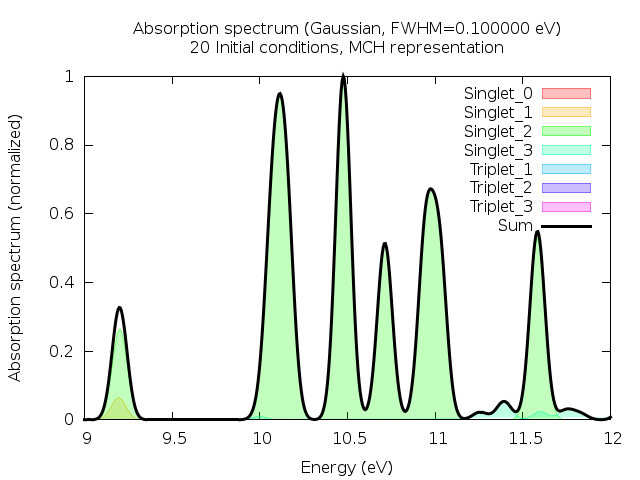
\includegraphics[width=0.75\textwidth]{figures/spectrum.png}
  \caption{Absorption spectrum and based on 10 initial conditions (Since there are 20 initial conditions in \ttt{initconds.excited}, the title lists 20 instead of 10).}
  \label{fig:spectrum}
\end{figure}











\clearpage
\section{Setting up dynamics simulations}

The last preparatory step towards dynamics simulations consists naturally in setting up the \sharc\ input files and run scripts. The interactive script \ttt{setup\_traj.py} takes care of this step. Run the script in the directory where the trajectories should be set up. Make sure that you have all files required by the interface (\ttt{MOLPRO.template}, \ttt{wf}) at hand.
\begin{Verbatim}[commandchars=\\\{\}]
user@host> \textcolor{red}{$SHARC/setup_traj.py}
\end{Verbatim}

\begin{oframed}
\footnotesize\begin{Verbatim}[commandchars=\\\{\}]
  ================================================================================
||                                                                                ||
||                      Setup trajectories for SHARC dynamics                     ||
||                                                                                ||
||                              Author: Sebastian Mai                             ||
||                                                                                ||
||                                   Version:0.2                                  ||
||                                    03.06.14                                    ||
||                                                                                ||
  ================================================================================


This script automatizes the setup of the input files for SHARC dynamics. 

  ================================================================================
||                               Initial conditions                               ||
  ================================================================================

This script reads the initial conditions (geometries, velocities, initial excited state)
from the initconds.excited files as provided by excite.py. 

Initial conditions file "initconds.excited" detected. Do you want to use this?
Use file "initconds.excited"? [True] \textcolor{red}{\textbf{<ENTER>}}

File initconds.excited contains 20 initial conditions.
Number of atoms is 6
Reference energy -78.081394900000 a.u.
Excited states are in MCH representation.

Please enter the number of states as a list of integers
e.g. 3 0 3 for three singlets, zero doublets and three triplets.
Number of states: [2 0 1] \textcolor{red}{\textbf{<ENTER>}}        \textcolor{blue}{# a different number of states than in the}
                                         \textcolor{blue}{# initial calculations could be used in the dynamics}
Number of states: [2, 0, 1]
Total number of states: 5

Do you want all states to be active? [True] \textcolor{red}{\textbf{<ENTER>}}

Do you want to see the content of the initconds file? [True] \textcolor{red}{\textbf{<ENTER>}}

Number of initial conditions in file:          20
Contents of the initconds file:

Legend:
?       Geometry and Velocity
.       not selected
#       selected

State 1:        \textcolor{blue}{# we performed only 10 initial excitation calculations, hence the "?"}
             10         20
              |          |
 0 | .......... ??????????       \textcolor{blue}{# No initial conditions selected in S0}
State 2:
             10         20
              |          |
 0 | ########## ??????????       \textcolor{blue}{# Initial conditions 1 to 10 are selected}
State 3:
             10         20
              |          |
 0 | .......... ??????????       \textcolor{blue}{# No initial conditions selected in T1}
State 4:
             10         20
              |          |
 0 | .......... ??????????
State 5:
             10         20
              |          |
 0 | .......... ??????????
Number of excited states and selections:
State    #InitCalc       #Selected
    1           10               0
    2           10              10        \textcolor{blue}{# we can setup 10 trajectories starting from state 2 (S1)}
    3           10               0
    4           10               0
    5           10               0

Please enter a list specifying for which excited states trajectories should be set-up
e.g. 1 2 5 to select states 1, 2, and 5.
States to setup the dynamics: [2] \textcolor{red}{\textbf{<ENTER>}}

There can be 10 trajectories set up.

Please enter the index of the first initial condition in the initconds file to be setup.
Starting index: [1] \textcolor{red}{\textbf{<ENTER>}}

There can be 10 trajectories set up, starting in 1 states.

Please enter the total number of trajectories to setup.
Number of trajectories: [10] \textcolor{red}{\textbf{<ENTER>}}

Please enter a random number generator seed (type "!" to initialize the RNG from the system time).
RNG Seed:  [!] \textcolor{red}{\textbf{1234}}


  ================================================================================
||                     Choose the quantum chemistry interface                     ||
  ================================================================================


Please specify the quantum chemistry interface (enter any of the following numbers):
1       MOLPRO (only CASSCF)
2       COLUMBUS (CASSCF, RASSCF and MRCISD), using SEWARD integrals
3       Analytical PESs
4       MOLCAS (only CASSCF)

Interface number: \textcolor{red}{\textbf{1}}



  ================================================================================
||                        Surface Hopping dynamics settings                       ||
  ================================================================================


-----------------------Simulation time----------------------

Please enter the total simulation time.
Simulation time (fs): [1000.0] \textcolor{red}{\textbf{100}}

Please enter the simulation timestep (0.5 fs recommended).
Simulation timestep (fs): [0.5] \textcolor{red}{\textbf{<ENTER>}}

Simulation will have 201 timesteps.

Please enter the number of substeps for propagation (25 recommended).
Nsubsteps: [25] \textcolor{red}{\textbf{<ENTER>}}

The trajectories can be prematurely terminated after they run for a certain time in 
the lowest state. 
Do you want to prematurely terminate trajectories? [False] \textcolor{red}{\textbf{<ENTER>}}


----------------------Dynamics settings---------------------

Do you want to perform the dynamics in the diagonal representation (SHARC dynamics) 
or in the MCH representation (regular surface hopping)?
SHARC dynamics? [True] \textcolor{red}{\textbf{<ENTER>}}

Please choose the quantities to describe non-adiabatic effects between the states:
1       DDT     =  < a|d/dt|b >        Hammes-Schiffer-Tully scheme   
2       DDR     =  < a|d/dR|b >        original Tully scheme          
3       overlap = < a(t0)|b(t) >       Local Diabatization scheme     

Coupling number: \textcolor{red}{\textbf{2}}

For SHARC dynamics, the evaluation of the mixed gradients necessitates to calculate 
non-adiabatic coupling vectors  (Recommended).
Include non-adiabatic couplings in the gradient transformation? [True]  \textcolor{red}{\textbf{<ENTER>}}

During a surface hop, the kinetic energy has to be modified in order to conserve total 
energy. There are several options to that:
1       Do not conserve total energy. Hops are never frustrated.
2       Adjust kinetic energy by rescaling the velocity vectors. Often sufficient.
3       Adjust kinetic energy only with the component of the velocity vector along the 
        non-adiabatic coupling vector.
EkinCorrect: [2]  \textcolor{red}{\textbf{<ENTER>}}

Do you want to apply decoherence to the diagonal states?
Decoherence? [True]  \textcolor{red}{\textbf{<ENTER>}}

Do you want to scale the energies and gradients?
Scaling? [False]  \textcolor{red}{\textbf{<ENTER>}}

Do you want to damp the dynamics (Kinetic energy is reduced at each timestep by a factor)?
Damping? [False]  \textcolor{red}{\textbf{<ENTER>}}



---------------Selection of Gradients and NACs--------------

In order to speed up calculations, SHARC is able to select which gradients and NAC vectors 
it has to calculate at a certain timestep. The selection is based on the energy difference 
between the state under consideration and the classical occupied state.

Select gradients? [False] \textcolor{red}{\textbf{yes}}                      \textcolor{blue}{# this and}
Select non-adiabatic couplings? [False] \textcolor{red}{\textbf{yes}}        \textcolor{blue}{# this strongly speeds up the calculation}

Please enter the energy difference threshold for the selection of gradients and 
non-adiabatic couplings (in eV). (0.5 eV recommended, or even larger if SOC is 
strong in this system.)
Selection threshold (eV): [0.5] \textcolor{red}{\textbf{<ENTER>}}


-------------------------Laser file-------------------------

Do you want to include a laser field in the simulation? [False] \textcolor{red}{\textbf{<ENTER>}}

  ================================================================================
||                             MOLPRO Interface setup                             ||
  ================================================================================


-----------------------Path to MOLPRO-----------------------

Environment variable $MOLPRO detected:
$MOLPRO=/usr/license/molpro/molpros_2012_1_5_Linux_x86_64_i8/bin//molpro

Do you want to use this MOLPRO installation? [True] \textcolor{red}{\textbf{<ENTER>}}

----------------------Scratch directory---------------------

Please specify an appropriate scratch directory. This will be used to temporally store the 
integrals. The scratch directory will be deleted after the calculation. Remember that this 
script cannot check whether the path is valid, since you may run the calculations on a 
different machine. The path will not be expanded by this script.
Path to scratch directory: (autocomplete enabled) \textcolor{red}{\textbf{$TMPDIR/Traj_WORK}}

-----------------MOLPRO input template file-----------------

Please specify the path to the MOLPRO.template file. This file must be a valid MOLPRO input 
file for a CASSCF calculation. It should contain the following settings:
- memory settings
- Basis set (possibly also Douglas-Kroll settings etc.)
- CASSCF calculation with:
  * Number of frozen, closed and occupied orbitals
  * wf and state cards for the specification of the wavefunction
MOLPRO.template files can easily be created using molpro_input.py (Open a second shell if you 
need to create one now).

The MOLPRO interface will generate the remaining MOLPRO input automatically.

Valid file "MOLPRO.template" detected. 
Use this template file? [True] \textcolor{red}{\textbf{<ENTER>}}

---------------Initial wavefunction: MO Guess---------------

Please specify the path to a MOLPRO wavefunction file containing suitable starting MOs for the 
CASSCF calculation. Please note that this script cannot check whether the wavefunction file 
and the Input template are consistent!

If you optimized your geometry with MOLPRO/CASSCF you can reuse the "wf" file from the 
optimization.

Do you have an initial wavefunction file? [True] \textcolor{red}{\textbf{<ENTER>}}
Initial wavefunction file: [wf.init] (autocomplete enabled) \textcolor{red}{\textbf{wf}}


  ================================================================================
||                                 Run mode setup                                 ||
  ================================================================================


-------------------------Run script-------------------------

This script can generate the run scripts for each trajectory in two modes:

  - In the first mode, the calculation is run in subdirectories of the current directory.

  - In the second mode, the input files are transferred to another directory (e.g. a local 
    scratch directory), the calculation is run there, results are copied back and the 
    temporary directory is deleted. Note that this temporary directory is not the same 
    as the scratchdir employed by the interfaces.

Note that in any case this script will setup the input subdirectories in the current 
working directory. 

Do you want to use mode 1 
(actually perform the calculations in subdirectories of: 
/user/mai/Documents/NewSHARC/SHARC_1.5/TESTS/Tutorial/MOLPRO_Ethylene)

Calculate here? [False] \textcolor{red}{\textbf{yes}}

----------------------Submission script---------------------

During the setup, a script for running all initial conditions sequentially in batch mode is 
generated. Additionally, a queue submission script can be generated for all initial conditions.

Generate submission script? [False] \textcolor{red}{\textbf{<ENTER>}}


#########################Full input#########################

ntraj                      10
ninit                      20
molpro.gradaccudefault     1e-07
states                     [2, 0, 1]
kill                       False
nstates                    5
molpro.guess               wf
show_content               True
eharm                      0.0543664278
n_issel                    [0, 10, 0, 0, 0]
nsubstep                   25
diag                       False
actstates                  [2, 0, 1]
ekincorrect                2
scratchdir                 $TMPDIR/Traj_WORK
eselect                    0.5
eref                       -78.0813949
damping                    False
firstindex                 1
cwd                        /user/sharc/Tutorial/Ethylene/
surf                       sharc
initf                      <open file 'initconds.excited', mode 'r' at 0x7f9c3f39d030>
dtstep                     0.5
repr                       MCH
here                       True
scaling                    False
statemap                   \{1: [1, 1,  0.0], 
                            2: [1, 2,  0.0], 
                            3: [3, 1, -1.0], 
                            4: [3, 1,  0.0], 
                            5: [3, 1,  1.0]\}
interface                  1
qsub                       False
laser                      False
coupling                   2
sel_g                      True
tmax                       100.0
molpro                     /usr/license/molpro/molpros_2012_1_5_Linux_x86_64_i8/bin//molpro
molpro.gradaccumax         0.01
sel_t                      True
setupstates                set([2])
printlevel                 2
natom                      6
gradcorrect                True
decoherence                0.1
molpro.template            MOLPRO.template
isactive                   [True, True, True, True, True]

Do you want to setup the specified calculations? [True] \textcolor{red}{\textbf{<ENTER>}}


  ================================================================================
||                            Setting up directories...                           ||
  ================================================================================


Progress: [==================================================] 100%

10 trajectories setup, last initial condition was 10 in state 2.
\end{Verbatim}
\end{oframed}

\normalsize

The script creates for each of the initial states (``States to setup the dynamics'') a directory called \ttt{<Mult>\_<Num>}, e.g., \ttt{Singlet\_1}, which contains the input for all trajectories starting in the $S_1$. 
Each of these directories contains subdirectories named \ttt{TRAJ\_00001}, \ttt{TRAJ\_00002}, etc. Note that these numbers are not consecutive: if an initial condition has not been selected, the number will be missing.
Each subdirectory contains the \sharc\ input (consisting of the files \ttt{input}, \ttt{geom}, and \ttt{veloc}), the directories \ttt{QM} and \ttt{restart}, and the run script for the trajectory, \ttt{run.sh}.

For the purposes of the tutorial it is sufficient to only calculate one trajectory. Change to the subdirectory of one of the trajectories and execute it.
\begin{Verbatim}[commandchars=\\\{\}]
user@host> \textcolor{red}{cd Singlet_1/TRAJ_00001}
user@host> \textcolor{red}{sh run.sh&}
user@host> \textcolor{red}{tailf output.lis}
\end{Verbatim}
While the trajectory is running, you can watch its progress in the file \ttt{output.lis} (short output listing). For each timestep, it contains the currently occupied diagonal state (and approximate MCH state), the kinetic, potential and total energy, the RMS gradient, the state dipole and spin expectation values of the currently occupied diagonal state and the time needed for this step. Surface hopping events are also mentioned in this file.

Besides the \ttt{output.lis} file, \sharc\ creates the files \ttt{output.log}, \ttt{output.xyz} and \ttt{output.dat}. The file
\ttt{output.log} contains mainly parsing information of the input file parsing and a list of internal steps of the dynamics simulation. With sufficiently high \ttt{printlevel} in the \sharc\ input file, the log file may also contain debug information in various detail.
The file \ttt{output.dat} contains for each timestep the most important matrices and vectors. This information can be used to calculate the excited-state energies, populations, hopping probabilities and a large number of expectation values. See below for the usage of \ttt{data\_extractor.x} and \ttt{make\_gnuplot.py}, which can be used for plotting the mentioned quantities.
Finally, \ttt{output.xyz} contains the cartesian coordinates of all atoms for each timestep. This file can be opened with any program capable of processing xyz files, like Molden, Molekel and Gabedit. Additionally, the \sharc\ suite contains the program \ttt{geo.py}, which is a command line tool to extract internal coordinates from such an xyz file.


% ===========================================================================================================================
% ===========================================================================================================================
% ===========================================================================================================================

% \chapter{Analysis of Trajectories}

We will first cover the analysis of a single trajectory based on the output files. Later we will also analyze ensemble properties. For these analysis the tutorial assumes that you ran trajectories \ttt{TRAJ\_00001} to \ttt{TRAJ\_00005}.

\section{Analyzing a single trajectory}

\subsection{Data extraction and plotting}

The file \ttt{output.dat} contains the Hamiltonian, transformation matrix, dipole matrices, coefficients, hopping probabilities, kinetic energy and random number from the surface hopping procedure in a compressed form. The program \ttt{data\_extractor.x} can be used to generate data tables, which can then be plotted.
\begin{Verbatim}[commandchars=\\\{\}]
user@host> \textcolor{red}{$SHARC/data_exctractor.x output.dat}
\end{Verbatim}
The program creates a subdirectory called \ttt{output\_data}. Currently, the following files will be created:
\begin{itemize}
  \item \ttt{coeff\_diag.out} contains the coefficients in the diagonal representation.
  \item \ttt{coeff\_MCH.out} contains the coefficients in the MCH representation.
  \item \ttt{energy.out} contains kinetic, current potential, total and potential energy of all excited states.
  \item \ttt{fosc.out} contains the oscillator strengths of the current state and all excited states.
  \item \ttt{spin.out} contains the total spin expectation values of the current state and all excited states.
  \item \ttt{expec.out} contains the content of \ttt{energy.out}, \ttt{fosc.out} and \ttt{spin.out} in one file (for plotting).
  \item \ttt{prob.out} contains the surface hopping random number and the hopping probabilities in the diagonal representation.
\end{itemize}

In order to plot the content of these files in an efficient manner, \ttt{gnuplot} can be used. Use
\begin{Verbatim}[commandchars=\\\{\}]
user@host> \textcolor{red}{$SHARC/make_gnuscript.py 2 0 1 > trajectory.gp}
\end{Verbatim}
to create a \ttt{gnuplot} script with the correct state numbering and labeling. Execute
\begin{Verbatim}[commandchars=\\\{\}]
user@host> \textcolor{red}{gnuplot trajectory.gp}
\end{Verbatim}
in the \ttt{output\_data} directory to plot energies, populations and hopping probabilities (Use \textcolor{red}{\ttt{<ENTER>}} to continue with the next plot). In figures~\ref{fig:en}, \ref{fig:cMCH}, \ref{fig:cDIAG} and~\ref{fig:prob} the output for ethylene trajectory \ttt{TRAJ\_00001} for the first 100~fs is given.

\begin{figure}[p]
  \centering
  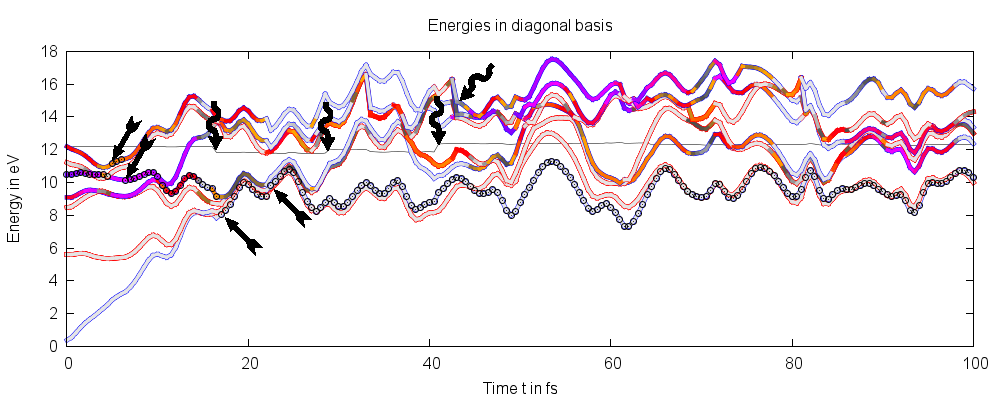
\includegraphics[width=\textwidth]{figures/energy.png}
  \caption{Plot of the potential energies for an ethylene trajectory with 2 singlet and 1 triplet states. }
  \label{fig:en}
\end{figure}
\begin{figure}[p]
  \centering
  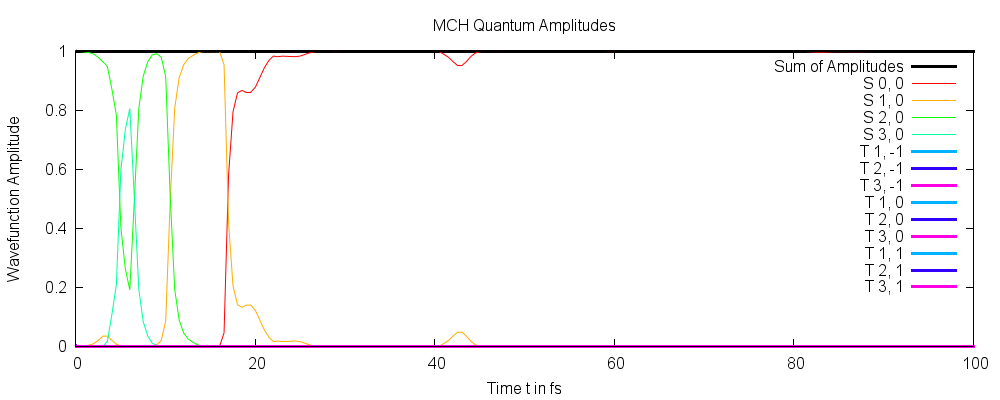
\includegraphics[width=\textwidth]{figures/coeff_MCH.png}
  \caption{Plot of the excited-state populations in the MCH representation.}
  \label{fig:cMCH}
\end{figure}
\begin{figure}[p]
  \centering
  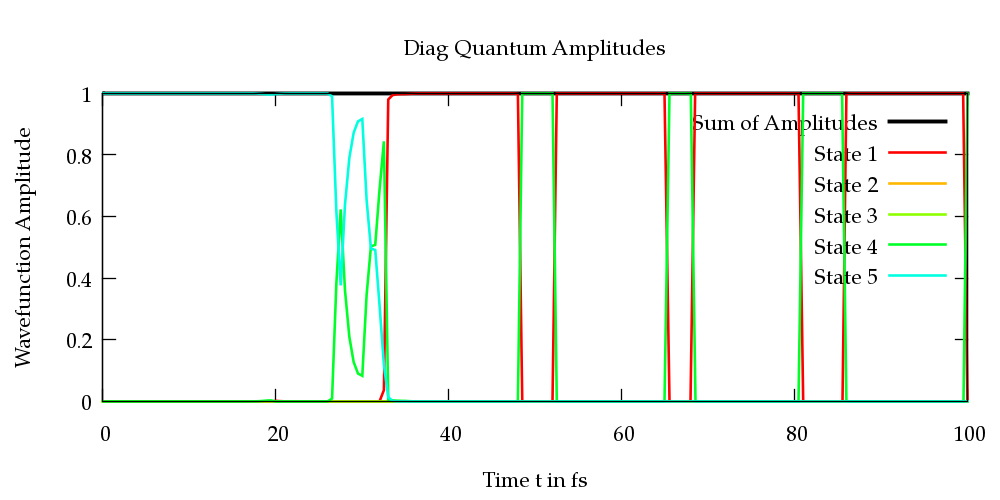
\includegraphics[width=\textwidth]{figures/coeff_diag.png}
  \caption{Plot of the excited-state populations in the diagonal representation.}
  \label{fig:cDIAG}
\end{figure}
\begin{figure}[p]
  \centering
  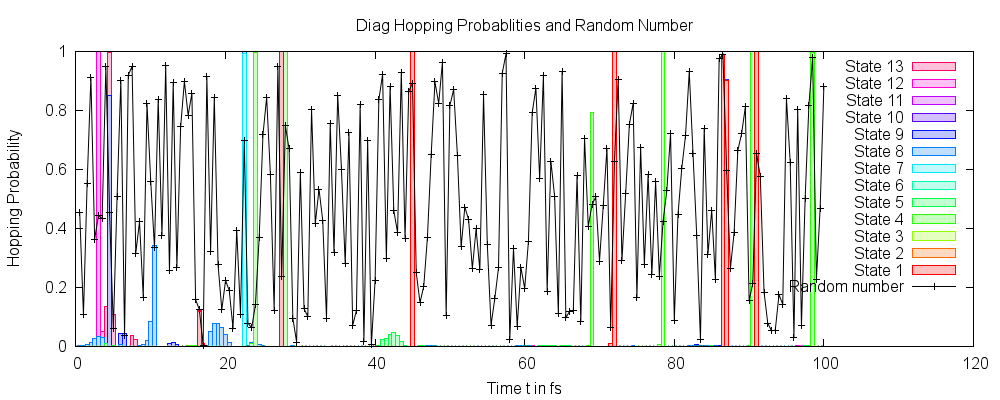
\includegraphics[width=\textwidth]{figures/prob.png}
  \caption{Plot of the hopping probabilities in the diagonal representation. Additionally, the random number for the surface hopping procedure is given.}
  \label{fig:prob}
\end{figure}

\paragraph{Discussion of Figure~\ref{fig:en}}

In figure~\ref{fig:en}, the potential energies of all states included in the dynamics depending on time is given. The currently occupied state is marked with black circles. Each line is is colored and additionally has a colored contour. The inner color encodes the oscillator strength of the state at each instant of time. Dark states are \textcolor{black!20}{light grey}, while brighter states are given in \textcolor{black!40}{grey}, \textcolor{black!70}{dark grey}, \textcolor{red!60!green}{orange}, \textcolor{red}{red}, \textcolor{red!50!blue}{magenta} or \textcolor{blue}{blue}, in order of increasing oscillator strength. The outer color encodes the total spin expectation value. Singlets are \textcolor{blue}{blue}, triplets \textcolor{red}{red} and states with mixed singlet-triplet character are \textcolor{green}{green}. Since in ethylene spin-orbit coupling is negligible, in the example only blue and red lines are visible.

In the figure, the trajectory starts in the highest excited state, which is singlet and very bright, according to the coloring. After some oscillations, at 30~fs it crosses with the lower singlet state and changes non-adiabatically to the lower state. For later times, the system oscillates with a lot of kinetic energy in the $S_0$. It also crosses with the $T_1$ on several occasions, notably around 50~fs, 65~fs and 80~fs. The thin black line at around 11~eV is the total energy of the system. It stays nearly constant, but fluctuates because the system has a lot of kinetic energy and the timestep is comparably large.

\paragraph{Discussion of Figure~\ref{fig:cMCH}}

In figure~\ref{fig:cMCH}, the MCH populations are given depending on time. The system starts with 100\% of the population in the upper singlet state $S_1$. Around 30~fs, population is transferred to $S_0$. The population transfer is complete at approximately 33~fs. In figure~\ref{fig:en} at the same time it can be seen that the trajectory switches to the lower singlet surface. In figure~\ref{fig:cMCH}, after the hop nearly 100\% of the population is in $S_0$. The triplet state does not get populated at all during the dynamics, which was expected, since the spin-orbit coupling is extremely weak and the singlet and triplet states do not stay close for long periods of time.

\paragraph{Discussion of Figure~\ref{fig:cDIAG}}

In figure~\ref{fig:cDIAG}, the diagonal populations are given depending on time. It can be seen nicely that the populated diagonal state changes several times during the simulation because the $S_0$ crosses with the $T_1$. In the diagonal representation, this leads to near-complete population transfer as $T_1$ becomes the lower state and $S_0$ the higher state (and vice versa).

\paragraph{Discussion of Figure~\ref{fig:prob}}

Figure~\ref{fig:prob} shows the surface hopping probabilities and the corresponding random numbers depending on time. In a nutshell, a surface hop happens whenever the random number lies within one of the colored bars. The color of the bar corresponds to the state into which the trajectory will hop. In the diagram, there are several hopping probabilities close to unity. This corresponds to the near-complete population transfer during the crossing of the $S_0$ and $T_1$ states. 




\clearpage
\subsection{Analyzing internal coordinates}

The file \ttt{output.xyz} contains the cartesian coordinates of all timesteps. Oftentimes, one is interested in the variation of certain internal coordinates (like bond lengths, angles, etc.) during the dynamics. The \sharc\ tool \ttt{geo.py} can quickly calculate these values. Invoke the program and enter the internal coordinate specifications:
\begin{Verbatim}[commandchars=\\\{\}]
user@host> \textcolor{red}{$SHARC/geo.py -g output.xyz -t 0.5}
\end{Verbatim}

\begin{oframed}
\footnotesize\begin{Verbatim}[commandchars=\\\{\}]
Enter the internal coordinate specifications:
\textcolor{red}{r 1 2}
\textcolor{red}{d 6 1 2 5}
\textcolor{red}{end}
Number of internal coordinate requests:   2
Number of geometries:    200
FINISHED!
\end{Verbatim}
\end{oframed}

\normalsize
The \ttt{-g} option specifies the filename of the input xyz geometry file, while the \ttt{-t} option specifies the timestep. \ttt{geo.py} writes the results to standard out, so redirect the output to some file:
\begin{Verbatim}[commandchars=\\\{\}]
user@host> \textcolor{red}{$SHARC/geo.py -g output.xyz -t 0.5 > Geo.out}
\end{Verbatim}
The file \ttt{Geo.out} contains a table with the specified internal coordinates:
\begin{oframed}
\footnotesize\begin{Verbatim}[commandchars=\\\{\}]
#                  1|                   2|                   3|
#               time|             r  1  2|       d  6  1  2  5|
              0.0000               1.3073              11.0993 
              0.5000               1.3157              10.1916 
              1.0000               1.3283               9.1573 
                   \vdots                    \vdots                    \vdots
\end{Verbatim}
\end{oframed}

Use \textsc{Gnuplot} to plot this table. 
\begin{Verbatim}[commandchars=\\\{\}]
user@host> \textcolor{red}{gnuplot}
\end{Verbatim}
The file \ttt{Geo.out} contains a table with the specified internal coordinates:
\begin{oframed}
\footnotesize\begin{Verbatim}[commandchars=\\\{\}]
gnuplot> \textcolor{red}{p "Geo.out" u 1:2 w l}     \textcolor{blue}{# Plot column 2 versus 1}
gnuplot> \textcolor{red}{p "Geo.out" u 1:3 w l}     \textcolor{blue}{# Plot column 3 versus 1}
\end{Verbatim}
\end{oframed}

\normalsize
The results are shown in figures \ref{fig:cc} and \ref{fig:dih}.

\paragraph{Discussion of the internal coordinates} 

In figures~\ref{fig:cc} the \ce{C=C} bond length is plotted over time. It can be easily seen that after excitation to the $\pi\pi^*$ state, the \ce{C=C} bond stretches strongly and starts to oscillate around the average bond length of a single \ce{C-C} bond (1.5 \AA). 

In figure~\ref{fig:dih}, the dihedral angle \ce{H-C=C-H} is plotted in degrees (confined to the interval $[0,180^\circ]$). It can be seen that after excitation the molecule undergoes torsion around the double bond. This (together with pyramidalization of the carbon atoms) leads to the well-known conical intersection of the $\pi\pi^*$ state and the ground state. In this trajectory, the conical intersection was reached after about 30~fs (recall figure~\ref{fig:en}).

\begin{figure}[h]
  \centering
  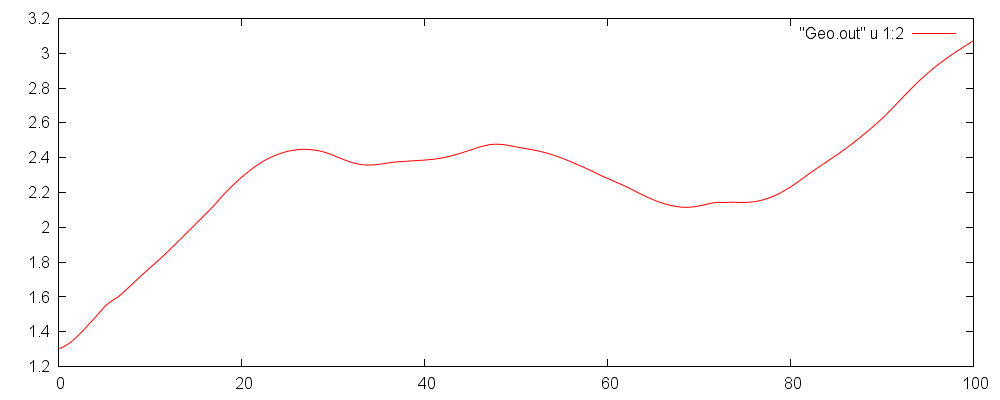
\includegraphics[width=\textwidth]{figures/CC.png}
  \caption{Value of the \ce{C=C} bond length during the simulation.}
  \label{fig:cc}
\end{figure}
\begin{figure}[h]
  \centering
  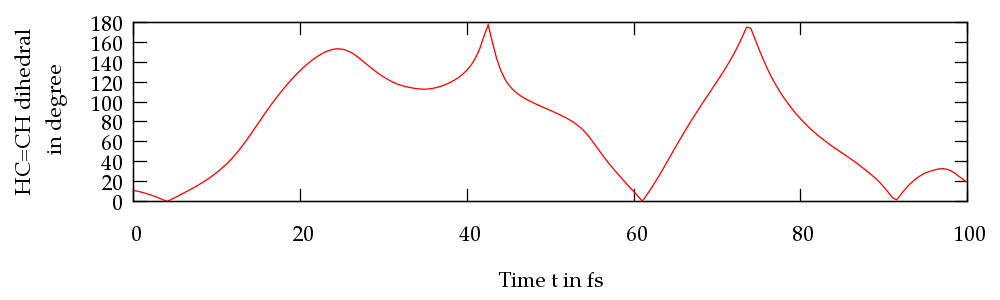
\includegraphics[width=\textwidth]{figures/dih.png}
  \caption{Value of one of the \ce{H-C=C-H} dihedrals during the simulation.}
  \label{fig:dih}
\end{figure}


\clearpage
\section{Analyzing the Ensemble}

\subsection{Ensemble Populations}

Among the main results of a \sharc\ simulation are the time-dependent excited-state populations within the simulated ensemble. In order to obtain these populations, the populations of all trajectories have to be summed up and normalized to the number of trajectories.

The script \ttt{populations.py} can be used to calculate various excited-state populations. There are several concepts:
\begin{itemize}
  \item Count for each timestep the number of trajectories in each classical state. These are the ``classical'' populations.
  \item For each timestep calculate the sum of the squares of the quantum amplitudes of each state. These sums are called the ``quantum'' populations.
  \item Count for each timestep the number of trajectories whose expectation values are within a certain interval. This can be used to obtain populations which correspond to certain classes of states (e.g.\ count all trajectories with large oscillator strength $\Rightarrow$ Approximate $\pi\pi^*$ population).
\end{itemize}

In the following, an example is given on the usage of \ttt{populations.py}, and afterwards the results of using the different concepts are discussed.

\begin{Verbatim}[commandchars=\\\{\}]
user@host> \textcolor{red}{$SHARC/populations.py}
\end{Verbatim}


% \subsection{Example}
% 
% This example shows how to obtain the classical populations for an ensemble of 5 ethylene trajectories.
% 
% If you want to exclude certain trajectories from the analysis, you can create an (empty) file called \ttt{CRASHED} in the directory of the trajectory. \ttt{populations.py} will skip trajectories where it finds a file called \ttt{CRASHED}, \ttt{RUNNING} or \ttt{DEAD}. 
\begin{oframed}
\footnotesize\begin{Verbatim}[commandchars=\\\{\}]
  ================================================================================  
||                                                                                ||
||                     Reading populations from SHARC dynamics                    ||
||                                                                                ||
||                              Author: Sebastian Mai                             ||
||                                                                                ||
||                                   Version:0.1                                  ||
||                                    12.03.14                                    ||
||                                                                                ||
  ================================================================================  

This script reads output.lis files and calculates ensemble populations 
(e.g. based on the classically occupied state or based on the quantum amplitudes).
  
--------------------Paths to trajectories-------------------

Please enter the paths to all directories containing the "TRAJ_0XXXX" directories.
E.g. S_2 and S_3. 
Please enter one path at a time, and type "end" to finish the list.
Path:  [end] (autocomplete enabled) \textcolor{red}{\textbf{Singlet_1}}
['TRAJ_00005', 'TRAJ_00004', 'TRAJ_00008', 'TRAJ_00001', 'TRAJ_00009', 
 'TRAJ_00002', 'TRAJ_00006', 'TRAJ_00010', 'TRAJ_00007', 'TRAJ_00003']
Found 10 subdirectories in total.

Path:  [end] (autocomplete enabled) \textcolor{red}{\textbf{<ENTER>}}

Total number of subdirectories: 10

------------------------Analyze Mode------------------------

This script can analyze the classical populations in different ways:
1       Number of trajectories in each diagonal state                                   
        from output.lis
2       Number of trajectories in each MCH state                                        
        from output.lis
3       Number of trajectories in each MCH state (multiplets summed up)                 
        from output.lis
4       Number of trajectories whose total spin value falls into certain intervals      
        from output.lis
5       Number of trajectories whose dipole moment falls into certain intervals         
        from output.lis
6       Number of trajectories whose oscillator strength falls into certain intervals   
        from output_data/fosc.out

It can also sum the quantum amplitudes:
7       Quantum amplitudes in diagonal picture                                          
        from output_data/coeff_diag.out
8       Quantum amplitudes in MCH picture                                               
        from output_data/coeff_MCH.out
9       Quantum amplitudes in MCH picture (multiplets summed up)                        
        from output_data/coeff_MCH.out

Analyze mode: \textcolor{red}{\textbf{3}}

----------------------Number of states----------------------

Please enter the number of states as a list of integers
e.g. 3 0 3 for three singlets, zero doublets and three triplets.
Number of states: [2 0 1] \textcolor{red}{\textbf{<ENTER>}}


------------------------Normalization-----------------------

Normalize the populations? [True] \textcolor{red}{\textbf{<ENTER>}}

-----------------------Simulation time----------------------

Up to which simulation time should the analysis be performed? (Trajectories 
which are shorter are continued with their last values.)
Simulation time (in fs):  [1000.0] \textcolor{red}{\textbf{100}}

-----------------------Gnuplot script-----------------------

Gnuplot script? [False] \textcolor{red}{\textbf{yes}}
Gnuplot script filename? [populations.gp] (autocomplete enabled) \textcolor{red}{\textbf{pop_class.gp}}

#########################Full input#########################

normalize                  True
paths                      ['Singlet_1/']
gnuplot_out                pop_class.gp
gnuplot                    True
run_extractor              False
states                     [2, 0, 1]
mode                       3
maxtime                    100.0
nstates                    3
nmstates                   5

Do you want to do the specified analysis? [True] \textcolor{red}{\textbf{<ENTER>}}

Checking the directories...          \textcolor{blue}{# If not all trajectories were run, this will be detected here}
Singlet_1//TRAJ_00005         OK
Singlet_1//TRAJ_00004         OK
Singlet_1//TRAJ_00008         Singlet_1//TRAJ_00008/output.lis NOT FOUND
Singlet_1//TRAJ_00001         OK
Singlet_1//TRAJ_00009         Singlet_1//TRAJ_00009/output.lis NOT FOUND
Singlet_1//TRAJ_00002         OK
Singlet_1//TRAJ_00006         Singlet_1//TRAJ_00006/output.lis NOT FOUND
Singlet_1//TRAJ_00010         Singlet_1//TRAJ_00010/output.lis NOT FOUND
Singlet_1//TRAJ_00007         Singlet_1//TRAJ_00007/output.lis NOT FOUND
Singlet_1//TRAJ_00003         OK
Number of trajectories: 5
Found dt=0.500000, nsteps=2001, nstates=3

Singlet_1//TRAJ_00005/output.lis                            200          \textcolor{blue}{# Number of steps read}
Singlet_1//TRAJ_00004/output.lis                            200
Singlet_1//TRAJ_00001/output.lis                            200
Singlet_1//TRAJ_00002/output.lis                            200
Singlet_1//TRAJ_00003/output.lis                            200
Shortest trajectory: 100.000000
Longest trajectory: 100.000000

Writing to pop.out ...
\end{Verbatim}
\end{oframed}

\normalsize
The incoherent sum of the quantum amplitudes can be calculated with mode 9. Rerun \ttt{populations.py}.
\begin{Verbatim}[commandchars=\\\{\}]
user@host> \textcolor{red}{$SHARC/populations.py}
\end{Verbatim}

\begin{oframed}
\footnotesize\begin{Verbatim}[commandchars=\\\{\}]
\vdots            \vdots            \vdots            \vdots            \vdots            \vdots            \vdots            

------------------------Analyze Mode------------------------

This script can analyze the classical populations in different ways:
1       Number of trajectories in each diagonal state                                   
        from output.lis
2       Number of trajectories in each MCH state                                        
        from output.lis
3       Number of trajectories in each MCH state (multiplets summed up)                 
        from output.lis
4       Number of trajectories whose total spin value falls into certain intervals      
        from output.lis
5       Number of trajectories whose dipole moment falls into certain intervals         
        from output.lis
6       Number of trajectories whose oscillator strength falls into certain intervals   
        from output_data/fosc.out

It can also sum the quantum amplitudes:
7       Quantum amplitudes in diagonal picture                                          
        from output_data/coeff_diag.out
8       Quantum amplitudes in MCH picture                                               
        from output_data/coeff_MCH.out
9       Quantum amplitudes in MCH picture (multiplets summed up)                        
        from output_data/coeff_MCH.out

Analyze mode: \textcolor{red}{\textbf{9}}

Run data_extractor.x for each trajectory prior to performing the analysis?
For many or long trajectories, this might take some time.
Run data_extractor.x? [True] \textcolor{red}{\textbf{<ENTER>}}

\vdots            \vdots            \vdots            \vdots            \vdots            \vdots            \vdots            

-----------------------Gnuplot script-----------------------

Gnuplot script? [False] \textcolor{red}{\textbf{yes}}
Gnuplot script filename? [populations.gp] (autocomplete enabled) \textcolor{red}{\textbf{pop_quant.gp}}

\vdots            \vdots            \vdots            \vdots            \vdots            \vdots            \vdots            

Overwrite pop.out?  [False] \textcolor{red}{\textbf{<ENTER>}}

Please enter the output filename:  (autocomplete enabled) \textcolor{red}{\textbf{pop_quant.out}}
Writing to pop_quant.out ...
\end{Verbatim}
\end{oframed}

\normalsize
Third, we obtain the number of trajectories whose oscillator strength falls into one of these intervals: $0<f_\text{osc}<10^{-4}$, $10^{-4}<f_\text{osc}<1^{-1}$ and $10^{-1}<f_\text{osc}$. Rerun \ttt{populations.py} again.
\begin{Verbatim}[commandchars=\\\{\}]
user@host> \textcolor{red}{$SHARC/populations.py}
\end{Verbatim}

\begin{oframed}
\footnotesize\begin{Verbatim}[commandchars=\\\{\}]
\vdots            \vdots            \vdots            \vdots            \vdots            \vdots            \vdots            

------------------------Analyze Mode------------------------

This script can analyze the classical populations in different ways:
1       Number of trajectories in each diagonal state                                   
        from output.lis
2       Number of trajectories in each MCH state                                        
        from output.lis
3       Number of trajectories in each MCH state (multiplets summed up)                 
        from output.lis
4       Number of trajectories whose total spin value falls into certain intervals      
        from output.lis
5       Number of trajectories whose dipole moment falls into certain intervals         
        from output.lis
6       Number of trajectories whose oscillator strength falls into certain intervals   
        from output_data/fosc.out

It can also sum the quantum amplitudes:
7       Quantum amplitudes in diagonal picture                                          
        from output_data/coeff_diag.out
8       Quantum amplitudes in MCH picture                                               
        from output_data/coeff_MCH.out
9       Quantum amplitudes in MCH picture (multiplets summed up)                        
        from output_data/coeff_MCH.out

Analyze mode: \textcolor{red}{\textbf{6}}

Run data_extractor.x for each trajectory prior to performing the analysis?
For many or long trajectories, this might take some time.
Run data_extractor.x? [True] \textcolor{red}{\textbf{no}}          \textcolor{blue}{# Was already done above}

\vdots            \vdots            \vdots            \vdots            \vdots            \vdots            \vdots            

-----------------------Gnuplot script-----------------------

Gnuplot script? [False] \textcolor{red}{\textbf{yes}}
Gnuplot script filename? [populations.gp] (autocomplete enabled) \textcolor{red}{\textbf{pop_fosc.gp}}

--------------------------Intervals-------------------------

Please enter the interval limits, all on one line.
Interval limits:  \textcolor{red}{\textbf{1e-4 1e-1}}          \textcolor{blue}{# Outer limits 0 and infinity are automatically assumed}

\vdots            \vdots            \vdots            \vdots            \vdots            \vdots            \vdots            

Overwrite pop.out?  [False] \textcolor{red}{\textbf{<ENTER>}}

Please enter the output filename:  (autocomplete enabled) \textcolor{red}{\textbf{pop_fosc.out}}
Writing to pop_quant.out ...
\end{Verbatim}
\end{oframed}

\normalsize
Use the produced \textsc{Gnuplot} scripts to plot the obtained populations.
\begin{Verbatim}[commandchars=\\\{\}]
user@host> \textcolor{red}{gnuplot pop_class.gp}
user@host> \textcolor{red}{gnuplot pop_quant.gp}
user@host> \textcolor{red}{gnuplot pop_fosc.gp}
\end{Verbatim}

This will create the files \ttt{pop\_class.gp.png}, \ttt{pop\_quant.gp.png} and \ttt{pop\_fosc.gp.png}. They are shown in figures~\ref{fig:pop_class}, \ref{fig:pop_quant} and \ref{fig:pop_fosc}. In \ref{fig:pop_class}, the classical populations are given. In figure~\ref{fig:pop_quant}, the incoherent sum of the quantum amplitudes is given (obtained by using mode 9 in \ttt{populations.py}). In figure~\ref{fig:pop_fosc}, the 5 trajectories are classified depending on their oscillator strengths.

\begin{figure}[p]
  \centering
  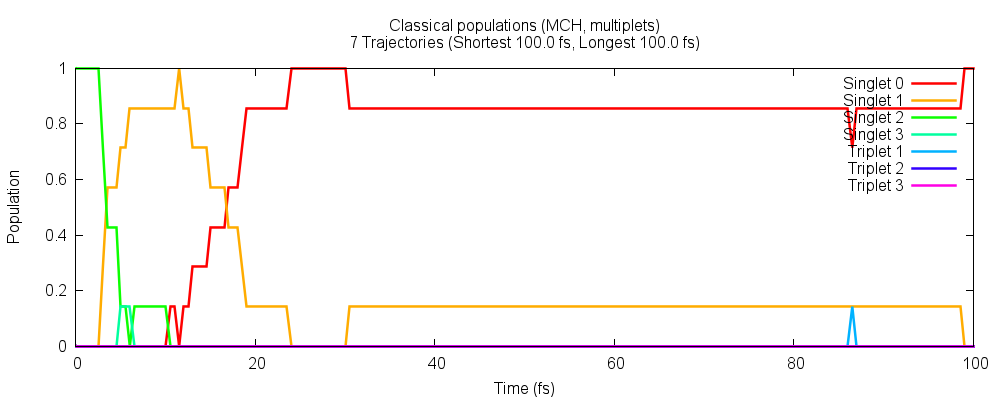
\includegraphics[width=\textwidth]{figures/pop_class.png}
  \caption{Classical populations for an ensemble of 5 trajectories.}
  \label{fig:pop_class}
\end{figure}
\begin{figure}[p]
  \centering
  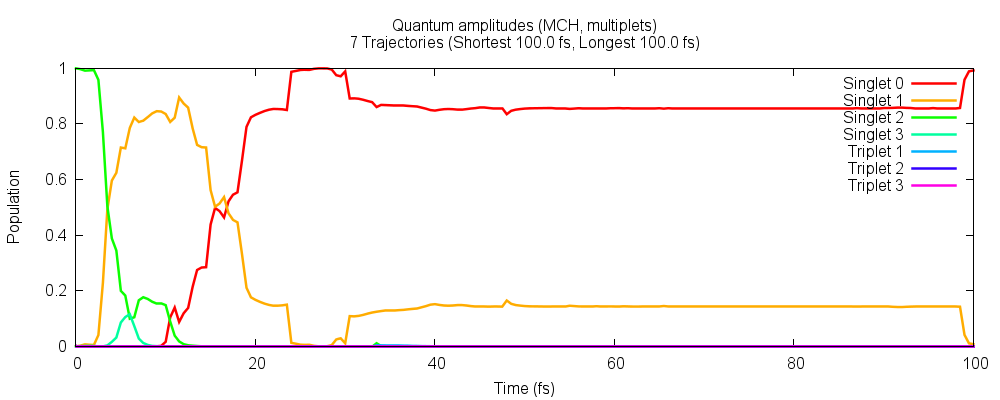
\includegraphics[width=\textwidth]{figures/pop_quant.png}
  \caption{Quantum populations for an ensemble of 5 trajectories.}
  \label{fig:pop_quant}
\end{figure}
\begin{figure}[p]
  \centering
  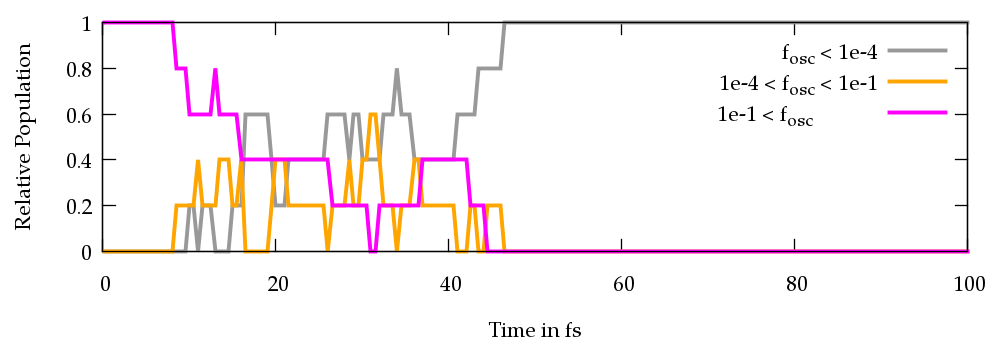
\includegraphics[width=\textwidth]{figures/pop_fosc.png}
  \caption{Populations classified based on oscillator strength for an ensemble of 5 trajectories.}
  \label{fig:pop_fosc}
\end{figure}



\paragraph{Discussion of Figure~\ref{fig:pop_class}}

In figure~\ref{fig:pop_class} it can be seen that between 30 and 50 fs simulation time, all ethylene trajectories changed from the initial $S_1$ state to the $S_0$ ground state. Two trajectories performed the surface hop at about 30 fs, while the remaining three trajectories switched between 40 and 50 fs. The $T_1$ state remained completely unpopulated. 

\paragraph{Discussion of Figure~\ref{fig:pop_quant}}

In figure~\ref{fig:pop_quant} the quantum populations are shown. For sufficiently large ensembles, figure~\ref{fig:pop_class} should closely follow figure~\ref{fig:pop_quant}. Consistency between the classical and quantum populations can be improved by using the decoherence correction (Input option in \ttt{setup\_traj.py}).

\paragraph{Discussion of Figure~\ref{fig:pop_fosc}}

In figure~\ref{fig:pop_fosc} the ensemble population was classified according to the oscillator strength of the classically populated state. The chosen interval limits were 0.0001 and 0.1, giving three classes of states (below 0.0001, between 0.0001 and 0.1, and above 0.1). Initially, all trajectories are in the bright $\pi\pi^*$ state and are thus classified into the third class. During the dynamics, the induced torsion around the double bond reduces the oscillator strength, so that the trajectories are classified into the intermediate class. Later, the trajectories decay to the ground state, which has by definition an oscillator strength of zero (since $f_\text{osc}$ is proportional to the excitation energy). Note that in this example the ground state cannot be distinguished from the triplet state, which has negligible oscillator strength and thus would also be classified into the first class. In general, however, classifying the population according to oscillator strength sometimes allows to approximately obtain populations of $\pi\pi^*$ and $n\pi^*$ states.



\clearpage
\subsection{Hopping Geometries}

Oftentimes, one is also interested in geometries which fulfill certain criteria, e.g., geometries where surface hops occured. \ttt{crossing.py} is a script to collect those geometries from all trajectories. Its usage is comparable to \ttt{populations.py}.
\begin{Verbatim}[commandchars=\\\{\}]
user@host> \textcolor{red}{$SHARC/crossing.py}
\end{Verbatim}

\begin{oframed}
\footnotesize\begin{Verbatim}[commandchars=\\\{\}]
  ================================================================================
||                                                                                ||
||                 Reading hopping geometries from SHARC dynamics                 ||
||                                                                                ||
||                              Author: Sebastian Mai                             ||
||                                                                                ||
||                                   Version:0.2                                  ||
||                                    04.06.14                                    ||
||                                                                                ||
  ================================================================================

This script reads output.lis files and output.xyz files to produce a list of 
all geometries where certain surface hops (or other events) occured.
  
--------------------Paths to trajectories-------------------

Please enter the paths to all directories containing the "TRAJ_0XXXX" directories.
E.g. S_2 and S_3. 
Please enter one path at a time, and type "end" to finish the list.
Path:  [end] (autocomplete enabled) \textcolor{red}{\textbf{Singlet_1}}
['TRAJ_00005', 'TRAJ_00004', 'TRAJ_00008', 'TRAJ_00001', 'TRAJ_00009', 
'TRAJ_00002', 'TRAJ_00006', 'TRAJ_00010', 'TRAJ_00007', 'TRAJ_00003']
Found 10 subdirectories in total.

Path:  [end] (autocomplete enabled) \textcolor{red}{\textbf{<ENTER>}}

Total number of subdirectories: 10

------------------------Analyze Mode------------------------

This script can find geometries where:
1        A change of MCH state occured (ignoring hops within one multiplet)
         from output.lis

Analyze mode: \textcolor{red}{\textbf{1}}

----------------------Number of states----------------------

Please enter the number of states as a list of integers
e.g. 3 0 3 for three singlets, zero doublets and three triplets.
Number of states: [2 0 1] \textcolor{red}{\textbf{<ENTER>}}

---------------States involved in surface hop---------------
In this analysis mode, all geometries are fetched where a trajectory 
switches from a given MCH state to another given MCH state.

Please enter the first MCH state involved (mult state):
State 1: \textcolor{red}{\textbf{1 2}}          \textcolor{blue}{# Only hops from S1}

Please enter the second MCH state involved (mult state):
State 2: \textcolor{red}{\textbf{1 1}}          \textcolor{blue}{# to S0}

Direction:
1       Forwards          \textcolor{blue}{# Only hops S1 -> S0}
2       Backwards         \textcolor{blue}{# Only hops S0 -> S1}
3       Two-way           \textcolor{blue}{# Hops S0 -> S1 and S1 -> S0}

Direction mode: [3] \textcolor{red}{\textbf{1}}

#########################Full input#########################

paths                      ['Singlet_1/']
tostates                   [[1, 1]]
run_extractor              False
states                     [2, 0, 1]
mode                       1
dirmode                    1
nstates                    3
fromstates                 [[1, 2]]
nmstates                   5

Do you want to do the specified analysis? [True] \textcolor{red}{\textbf{<ENTER>}}

Checking the directories...
Singlet_1//TRAJ_00001         OK
Singlet_1//TRAJ_00002         OK
Singlet_1//TRAJ_00003         OK
Singlet_1//TRAJ_00004         OK
Singlet_1//TRAJ_00005         OK
Singlet_1//TRAJ_00006         Singlet_1//TRAJ_00006/output.lis NOT FOUND
Singlet_1//TRAJ_00007         Singlet_1//TRAJ_00007/output.lis NOT FOUND
Singlet_1//TRAJ_00008         Singlet_1//TRAJ_00008/output.lis NOT FOUND
Singlet_1//TRAJ_00009         Singlet_1//TRAJ_00009/output.lis NOT FOUND
Singlet_1//TRAJ_00010         Singlet_1//TRAJ_00010/output.lis NOT FOUND
Number of trajectories: 5

Writing to crossing.xyz ...
\end{Verbatim}
\end{oframed}

\normalsize
The output file \ttt{crossing.xyz} in turn can also be analyzed with \ttt{geo.py} in order to calculate internal coordinates. 







\chapter{Specialized Tutorials}

\section{Using non-default atomic masses}

Sometimes, in dynamics simulations one is interested in isotope effects. This necessitates the modification of the atomic mass of the corresponding atoms. The atomic masses are included in the geometry file, which is read by \sharc\ during initialization of the dynamics.

Furthermore, modification of the atomic masses influences the Wigner distribution of initial conditions. \ttt{wigner.py} has a facility to adjust the atomic mass during initial condition generation. Call \ttt{wigner.py} as usual, but include the \ttt{-m} option:
\begin{Verbatim}[commandchars=\\\{\}]
user@host> \textcolor{red}{$SHARC/wigner.py freq.molden -m}
\end{Verbatim}

Instead of directly producing the initial conditions file, \ttt{wigner.py} will start a dialog, where the user can modify the atomic masses. Initially, all atoms are assumed to use the default mass (the mass of the most common isotope). The user can then add atoms to the list of atoms with non-default masses, thereby specifying the mass. 
\begin{oframed}
\footnotesize\begin{Verbatim}[commandchars=\\\{\}]
Initial condition generation started...
MOLDEN file                  = "freq.molden"
OUTPUT file                  = "initconds"
Number of geometries         = 20
Random number generator seed = 16661

Option -m used, please enter non-default masses:
+ number mass           add non-default mass <mass> for atom <number>
- number                remove non-default mass for atom <number> (default mass will be used)
show                    show non-default atom masses
end                     finish input for non-default masses

\textcolor{red}{\textbf{+ 1 14.054321}}         \textcolor{blue}{# Give atom number 1 the mass 14.054321}
\textcolor{red}{\textbf{show}}
-----------------------
Atom               Mass
   1    14.054321000000
-----------------------
\textcolor{red}{\textbf{- 1}}                   \textcolor{blue}{# Give atom number 1 the default mass}
\textcolor{red}{\textbf{+ 2 16.054321}}         \textcolor{blue}{# Give atom number 2 the mass 16.054321}
\textcolor{red}{\textbf{+ 2 15.054321}}         \textcolor{blue}{# Give atom number 2 the mass 15.054321}
\textcolor{red}{\textbf{end}}
Geometry:
 C   6.0  -0.00000000   0.00000000  -0.00760978  12.00000000 
 C   6.0   0.00000000   0.00000000   2.53039416  15.05432100 
 H   1.0   1.73012211   0.00000000  -1.07271869   1.00782503 
 H   1.0   1.73012212   0.00000000   3.59550308   1.00782503 
 H   1.0  -1.73012211   0.00000000   3.59550308   1.00782503 
 H   1.0  -1.73012212   0.00000000  -1.07271870   1.00782503 
Assumed Isotopes: H-1 C-12 
Isotopes with * are pure isotopes.

Frequencies (cm^-1):
   1     885.9700
   2     970.0600
   3    1068.5700
   4    1299.2900
   5    1342.3400
   6    1439.6100
   7    1605.6600
   8    1774.6800
   9    3319.3700
  10    3339.1300
  11    3396.7200
  12    3422.7000

\end{Verbatim}
\end{oframed}

\normalsize
Note that with the \ttt{+} command the mass of an already specified atom can also be changed. 

\paragraph{Frequency calculation}

Please also note that the preceeding frequency calculation also has to use the same atomic masses as the run of \ttt{wigner.py}. For \textsc{Molpro}, \ttt{molpro\_input.py} can setup frequency calculations with non-standard atomic masses. For \textsc{Columbus}, the user can edit the \ttt{geom} before starting the frequency calculation.


\section{Inactive states}

Sometimes, states should be included in the dynamics simulation in order to calculate transient absorption spectra, transient ionization spectra or simply in order to see how these states evolve during the dynamics. When it is not expected that these states are actually occupied during the simulation, \sharc\ has a mechanism to neglect all couplings between these states (called inactive henceforth) and the occupied states. This allows also to neglect the gradients and non-adiabatic couplings involving these states, thereby saving considerable amounts of computation time. 

It is only possible to make the highest states in each multiplicity inactive. With \ttt{states 3 0 3} and \ttt{actstates 2 0 1} in the \sharc\ input, one would include $S_0$, $S_1$, $S_2$, $T_1$, $T_2$ and $T_3$ in the simulation, but restrict the actual dynamics to $S_0$, $S_1$ and $T_1$.

It is advisable to make inactive all states which do not show any couplings with the occupied states (e.g., ionic states in a dynamics simulation of a neutral molecule). 

\paragraph{Inactive states in \ttt{excite.py}}

\ttt{excite.py} also allows to exclude states in the excitation process. Note, however, that this is unrelated to the inactive states in the dynamics. It would be possible to exclude a state in the excitation process but still keep it in the dynamics simulation. An example would be to excite to dark $n\pi^*$ states, which would not be selected if bright $\pi\pi^*$ states are present.


\section{Ionization spectra using \ttt{excite.py} and the \textsc{Columbus} interface}

When using the \textsc{Columbus} interface, it is possible to calculate Dyson norms between pairs of neutral and ionic states. These norms are an estimate for the single-photon ionization probability. \ttt{setup\_init.py} and \ttt{excite.py} can be used to calculation ionization spectra based on a Wigner distribution of geometries, essentially in the same way as absorption spectra are calculated.

\subsection{\ttt{setup\_init.py} Input}

First, obtain the \ttt{initconds} file as usual. Then setup the initial excited-state calculations. Use the \textsc{Columbus} interface. The last interface-related question will be whether Dyson norms should be calculated. Enter the path to the Dyson program of Matthias Ruckenbauer and to the Dyson-compatible version of \ttt{civecconsolidate}.
\begin{oframed}
\footnotesize\begin{Verbatim}[commandchars=\\\{\}]
------------Ionization probability by Dyson norms-----------

Dyson norms? [False] \textcolor{red}{\textbf{yes}}
Path to dyson executable: (autocomplete enabled) \textcolor{red}{\textbf{$DYSON/dyson.x}}
Path to civecconsolidate executable: [$COLUMBUS/civecconsolidate] (autocomplete enabled) \textcolor{red}{\textbf{<ENTER>}}
c2 threshold for Dyson: [0.0001] \textcolor{red}{\textbf{<ENTER>}}
\end{Verbatim}
\end{oframed}

\normalsize
Finish the setup as usual and run the calculations.

\subsection{\ttt{excite.py} Input}

Use \ttt{excite.py} as usual to read the results of the excited-state calculations. Near the end, the following question is asked:
\begin{oframed}
\footnotesize\begin{Verbatim}[commandchars=\\\{\}]
Use Dyson norms instead of dipole moments? [False] \textcolor{red}{\textbf{yes}}
\end{Verbatim}
\end{oframed}

\normalsize
The script will use the Dyson norms in the place of the $x$ component of the transition dipole moments, while the $y$ and $z$ components will be set to zero. The remaining usage is identical to the regular case (transition dipole moments). \ttt{spectrum.py} can be used to obtain plottable spectra.

\chapter{Usage of the Interfaces}

All of the \sharc\ scripts are in principal compatible with the interfaces to \textsc{Molpro}, \textsc{Molcas} and \textsc{Columbus}. However, depending on the interface, some details of the preparation of the dynamics change. In the following, these details are adressed.

\section{MOLPRO}

See the full tutorial in chapter \ref{chap:full}. In combination with \ttt{molpro\_input.py} and the setup scripts, usage should be relatively straight-forward.

\section{MOLCAS}

Instead of the \ttt{MOLPRO.template} file needed for \textsc{Molpro}, usage of \textsc{Molcas} requires a \ttt{MOLCAS.template} file, which has a different structure. The template file can be setup with the script \ttt{molcas\_input.py}.

\subsection{Template file}

An examplary template file looks like:
\begin{oframed}
\footnotesize\begin{Verbatim}[commandchars=\\\{\}]
basis cc-pvdz
ras2 3
nactel 4
inactive 6
spin 1 roots 4
spin 3 roots 3
\end{Verbatim}
\end{oframed}

Currently, there are no more keywords than the ones given in this example. \ttt{basis} defines the basis set, \ttt{ras2} is the number of active orbitals, \ttt{nactel} is the number of active electrons and \ttt{inactive} is the number of doubly occupied orbitals. 
The lines with \ttt{spin} and \ttt{roots} keywords defines the number of states per multiplicity, in this case 4 singlet states and 3 triplet states.

\section{COLUMBUS}

Since \textsc{Columbus} is a complex suite of many independent programs (each with own input files), input preparation is conducted with \textsc{Columbus}' interactive input facility \ttt{colinp}. In order to perform single-point calculations and optimizations/frequency calculations, please refer to the 
\href{http://www.univie.ac.at/columbus/docs_COL70/documentation_main.html}{\textsc{Columbus} online documentation} and the 
\href{http://www.univie.ac.at/columbus/docs_COL70/tutorial.pdf}{standard tutorial}.

\subsection{General steps in running COLUMBUS}

In order to use \textsc{Columbus}, whether via its driver script \ttt{runc} or through the \sharc-\textsc{Columbus} interface, you have to set the environment variable \ttt{\$COLUMBUS} to the directory containing the \textsc{Columbus} executables (like \ttt{runc}, \ttt{mcscf.x}, \ttt{ciudg.x}, etc.).

In order to prepare a calculation, first convert the standard xyz file containing the molecular geometry to \textsc{Columbus} format:
\begin{verbatim}
user@host> $COLUMBUS/xyz2col.x < geom.xyz
\end{verbatim}
which will create the file \ttt{geom}. Then, start \ttt{colinp}
\begin{verbatim}
user@host> $COLUMBUS/colinp
\end{verbatim}

Go through the input sections, starting with the integral section, followed by SCF, CASSCF, MRCI and finally the run setup. After the preparation of the input, start \textsc{Columbus} via
\begin{verbatim}
user@host> $COLUMBUS/runc -m [MEMORY in MB] > runls&
\end{verbatim}
An optimization can be carried out directly with \ttt{runc} -- just use the corresponding options in \ttt{colinp}.

For a (numerical) frequency calculation, use \ttt{colinp} to generate the internal coordinates and the \ttt{DISPLACEMENT} directories. Then, a calculation needs to be carried out in each of the \ttt{DISPLACEMENT} subdirectories, a task which is accomplished by the \ttt{calc.pl} script. The script \ttt{forceconst.pl} collects the results and produces the file \ttt{suscalls}, which is compatible with the MOLDEN format (and can be used with \ttt{wigner.py}).

\subsection{COLUMBUS input for usage with the interface}

Instead of a template file as in the \textsc{Molpro} case, for \textsc{Columbus} a template directory is needed.
The directory contains one subdirectory with input for each multiplicity (singlets, doublets, triplets, \dots). However, even-electron wavefunctions of different multiplicities can be computed together in the same job if spin-orbit couplings are desired. Otherwise independent multiple-DRT inputs (ISC keyword) are also acceptable. Note that symmetry is not allowed when using the interface.

In order to prepare the input for the \sharc-\textsc{Columbus} interface, you can furthermore see the 
\href{http://www.univie.ac.at/columbus/docs_COL70/tutorial-SO.pdf}{tutorial on spin-orbit coupling calculations}.

\paragraph{Integral input}

The interface is only able to use input for calculations using \textsc{Molpro/Seward} integrals. No symmetry is allowed here. Make sure that you include scalar-relativistic and spin-orbit (AMFI) effects in the integral input. 

\paragraph{MCSCF input}

The MCSCF section can use any desired state-averaging scheme. However, frozen core orbitals in the MCSCF step are not possible. Prepare the MCSCF input for CI gradients. It is advisable to use very tight MCSCF convergence criteria.

\paragraph{MRCI input}

Either prepare a single-DRT input without SOCI (to cover a single multiplicity), a single-DRT input with SOCI and a sufficient maximum multiplicity for spin-orbit couplings or a independent multiple-DRT input (ISC case). Make sure that all multiplicities are covered with all input directories.

In the MRCI input, make sure to use sequential \ttt{ciudg}. Also take care to setup gradient input on MRCI level.

\paragraph{Job control}

Setup a single-point calculation with the following steps:
\begin{itemize}
  \item SCF
  \item MCSCF
  \item MR-CISD (serial operation) or SO-CI coupled to non-rel CI (for SOCI DRT inputs)
  \item one-electron properties for all methods
  \item transition moments for MR-CISD
  \item nonadiabatic couplings (and/or gradients)
\end{itemize}

Request first transition moments and interstate couplings in the following dialogues. Analysis in internal coordinates and intersection slope analysis are not required.



\section{Analytical expressions}

For the interface using analytical expressions for the potential energy surfaces, only one input file (\ttt{SH2Ana.inp}) is needed. This file contains the definitions of all analytical expressions. See below for an example of this file.

The remaining procedure with the analytical potential interface is analogue to the usage of the other interfaces.

\subsection{One-dimensional case}

In the following, we will prepare the input for a single particle moving in one dimension on two states.

The file \ttt{SH2Ana.inp} consists of a file header and a file body. The header for the one-dimensional case and for two states could look as follows:
\begin{oframed}
\footnotesize\begin{Verbatim}[commandchars=\\\{\}]
1
2
H       x       0       0
\end{Verbatim}
\end{oframed}
The first line defines the number of atoms to be one, the second line gives the number of states. The third line is a mapping of the cartesian coordinates of the atom to variable names. In this case, the $x$ component of the coordinate of the atom is linked to the actual variable called \ttt{x}. The variable can then be used in the file body in the definitions of the potentials.

Below the file header (with $n_\text{atom}+2$ lines), different blocks can be put. Variable blocks define can be used to define constants:
\begin{oframed}
\footnotesize\begin{Verbatim}[commandchars=\\\{\}]
Variables
k 2.0
D12 10.0
Re 2.0
omega 13.
mu 1.0
End
\end{Verbatim}
\end{oframed}

Most importantly, matrix blocks define the potential energies, couplings and gradients. A matrix block could look like:
\begin{oframed}
\footnotesize\begin{Verbatim}[commandchars=\\\{\}]
Hamiltonian
0.5*k*x**2+omega,
0,   0.5*k*(x-Re)**2+D12,
\end{Verbatim}
\end{oframed}
Note the keyword \ttt{Hamiltonian}, which defines the type of matrix given.

Another matrix block gives the derivatives of the Hamiltonian with respect to the variable \ttt{x}:
\begin{oframed}
\footnotesize\begin{Verbatim}[commandchars=\\\{\}]
Derivatives     x
k*x,
0,   k*(x-Re),
\end{Verbatim}
\end{oframed}
The user has to provide the correct derivatives of the Hamiltonian manually.

Put together, the complete input for the example might look like:
\begin{oframed}
\footnotesize\begin{Verbatim}[commandchars=\\\{\}]
1
2
H       x       0       0

Variables
k 2.0
D12 10.0
Re 2.0
mu 1.0
End

Hamiltonian
0.5*k*x**2,
0,   0.5*k*(x-Re)**2+D12,

Derivatives     x       \textcolor{blue}{# Derivatives with respect to x}
k*x,                    \textcolor{blue}{# Derivatives need to be given manually}
0,   k*(x-Re),

Dipole  1
0.0,
0.5*mu, 0.0,

\end{Verbatim}
\end{oframed}

Only the \ttt{Hamiltonian} block and one \ttt{Derivatives} block for each variable needs to be present. Optional blocks are \ttt{SpinOrbit}, \ttt{Dipole} and \ttt{Dipolederivaties}. 

For more details please refer to the manual.











\end{document}
